% \documentclass[../document.tex]{subfiles}
% \begin{document}
\section{Test dataset exploration}
\label{sec: quarry-dataset}
After showing the model's capability of correctly separate classes' features we utilized Grad-CAM to visualize some patches inside the quarry dataset. The aim of this section is to show how the model looks at meaningful features in each input to make the prediction even when it fails. For instance, imagine we feed to the model a not traversable patch with an obstacle and the network label is as traversable. Clearly, the output is wrong but the model's error may be caused by two different situations. The first one, the model could just have ignored the obstacle and looked away, meaning that it was not even able to understand there was an obstacle in the first place. Second, the network could have correctly look at the obstacle but thought that obstacle is traversable, showing the correct ability to find and use important features in the map. In the following sections, we showed that, even when the predictions are wrong, our model always look at the most important features of each input to determine its traversability. 

We divided the dataset patches into four classes based on the model's performance: worst, best, false positive and false negative. Then, we took twenty inputs from these sets and applied a technique called Grad-CAM to visualize which part of the ground the model is looking. These regions are highlighted in 3D render to better visualize which spot of the inputs caused the prediction. Before starting the exploration, let us introduce the method that allowed us to identify regions of interest on the patches. 
% \subsection{Best}
% We start evaluating our model by using the test set composed by samples from the Quarry map. Grad-CAM is an extremely powerful tool to interpret the results in this situation since most of the patches are hard to classify even at humans eye since they include different features on the same surface.
\subsection{Grad-CAM}
Before starting the exploration, let us introduce the method used to identify region of interest on the patches. Gradient-weighted Class Activation Mapping (Grad-CAM) \cite{gradcam} is a technique to produce \"visual explanations\" for convolutional neural networks. It highlights the regions of the input image that contribute the most to the predictions. For example, given a classifier able to recognize cats and cat image, Grad-CAM will point outs the cat.
\begin{figure} [htbp]
    \centering
    \begin{subfigure}[b]{1\textwidth}
        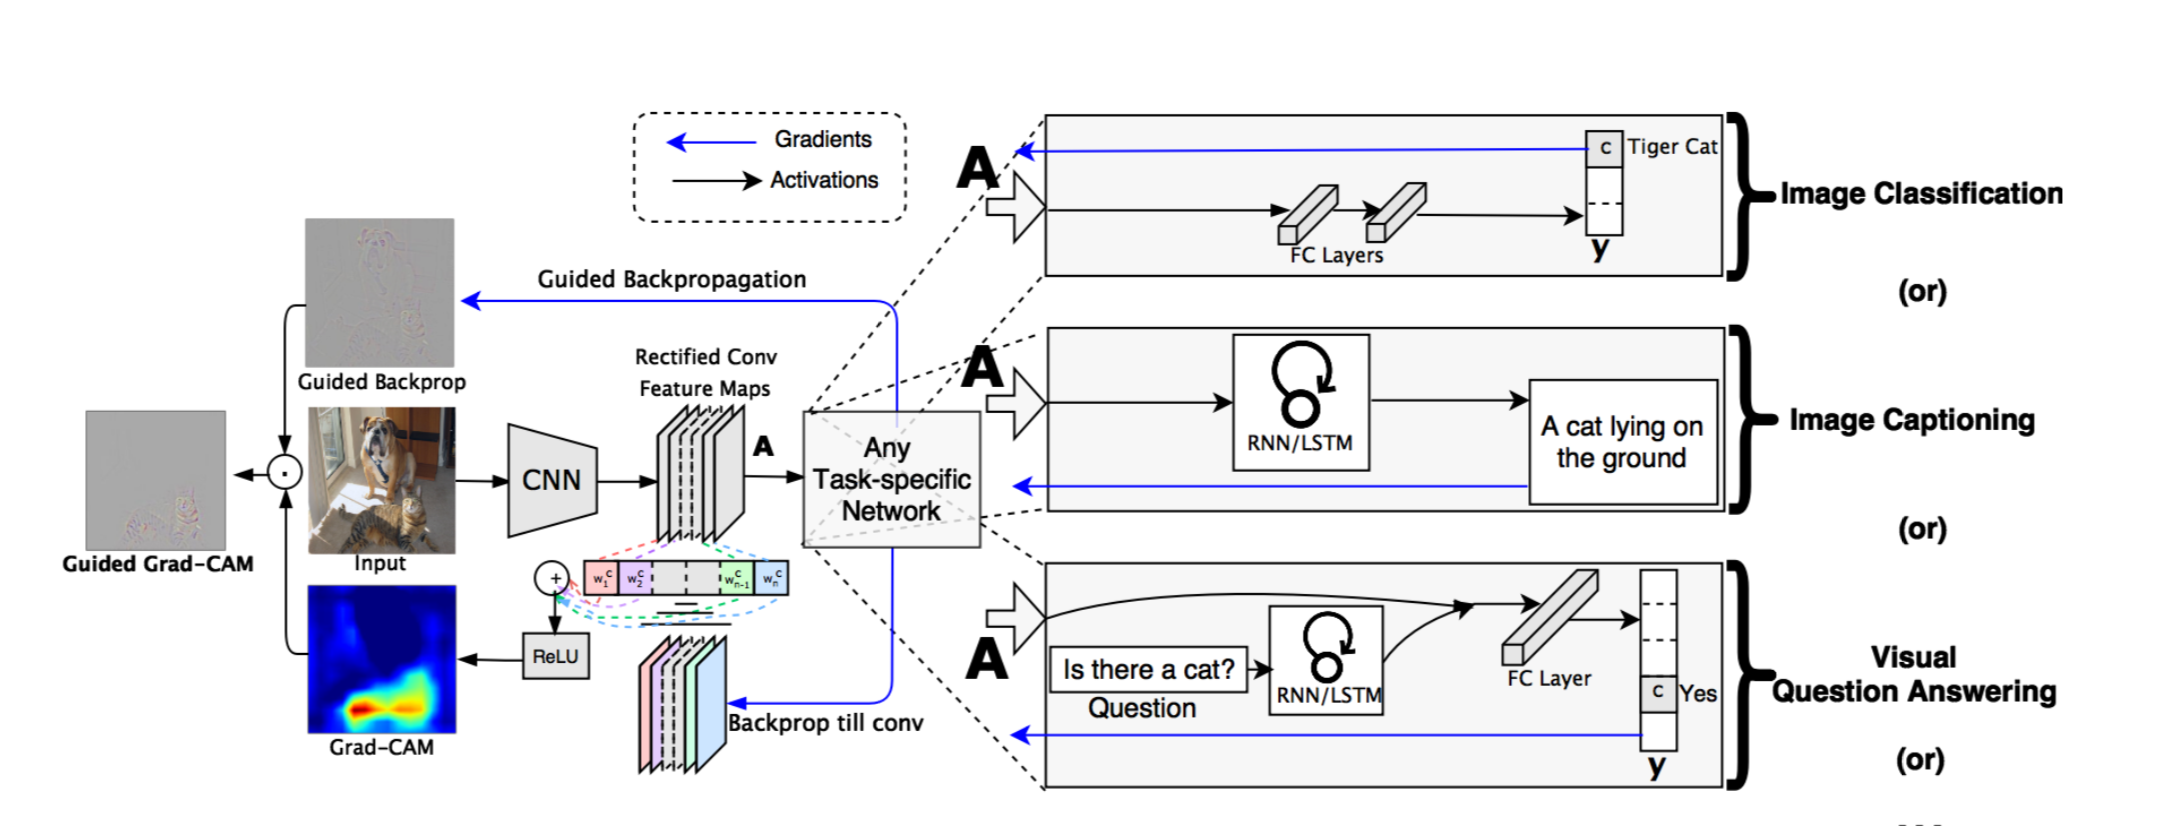
\includegraphics[width=\linewidth]{../img/5/grad_cam1.png}
    \end{subfigure}
\caption{Grad-CAM procedure on an input image. Image from the original paper \cite{gradcam}.}
\label{fig: gradcam}
\end{figure}
In detail, the output with respect to a target class is backpropagated while storing the gradient and the last convolution layer's output. Then, a global average is applied to the saved gradient keeping the channel dimension in order to get a 1-d tensor, this will represent the importance of each channel in the target convolutional layer. After, each element of the convolutional layer outputs is multiplied with the averaged gradients to create the grad cam. This whole procedure is fast and it is architecture independent. The procedure is summarized by figure \ref{fig : gradcam}

\subsection{Traversable patches}
These samples are the patches correctly predicted as traversable. We plotted twenty different inputs sampled uniformly according to the robot advancement to include as many interesting situations as possible. We recognized two main clusters of images: flat, figures \ref{fig : quarry-best-1},  \ref{fig : quarry-best-2},  \ref{fig : quarry-best-6},  \ref{fig : quarry-best-7},  \ref{fig : quarry-best-8},  \ref{fig : quarry-best-9},  \ref{fig : quarry-best-10},  \ref{fig : quarry-best-11},  \ref{fig : quarry-best-15},  \ref{fig : quarry-best-17},  \ref{fig : quarry-best-19}, and slopes, figures  \ref{fig : quarry-best-3},  \ref{fig : quarry-best-4},  \ref{fig : quarry-best-5},  \ref{fig : quarry-best-12},  \ref{fig : quarry-best-13},  \ref{fig : quarry-best-14},  \ref{fig : quarry-best-16},  \ref{fig : quarry-best-20}. The models is mostly interested in the left part of the patches with uneven ground on the left region, \ref{fig : quarry-best-1}, \ref{fig : quarry-best-2}, \ref{fig : quarry-best-3}, \ref{fig : quarry-best-4}, \ref{fig : quarry-best-5}, \ref{fig : quarry-best-7}, \ref{fig : quarry-best-10}, \ref{fig : quarry-best-12}, \ref{fig : quarry-best-13}, \ref{fig : quarry-best-14}, \ref{fig : quarry-best-15}, \ref{fig : quarry-best-16}, \ref{fig : quarry-best-18}. This is due to the fact that an obstacle in that region can block the rear legs and prevent the robot to advance. In other patches where most probably a untraversable features may also be present ahead, the model discriminates different parts of the map. For instance, figure \ref{fig : quarry-best-4} shows an interest region on the slope near the end and figure  \ref{fig : quarry-best-12} on two stop of the first faily big step ahead of the robot. Similarly, also figures  \ref{fig : quarry-best-14},  \ref{fig : quarry-best-17},  \ref{fig : quarry-best-19}.

In some situations, the model identify a possible untraversable spot only forward being sure the robot is no immeaditely stopped. There are two obvious cases, figures \ref{fig : quarry-best-8} ,  \ref{fig : quarry-best-9} and \ref{fig : quarry-best-19}. The first one is a totally flat surface, so the model looks as far as possible to check if there are obstacles. We have a similar situation in the last two patches, a surface with a some noise and a big bump respectively, where the network verifies these spots. So, rightly, the network analysis the first region of the patch that may contain an untraversable obstacle. 
\begin{figure}[H]
    \centering
    \begin{subfigure}[b]{0.192\linewidth}
    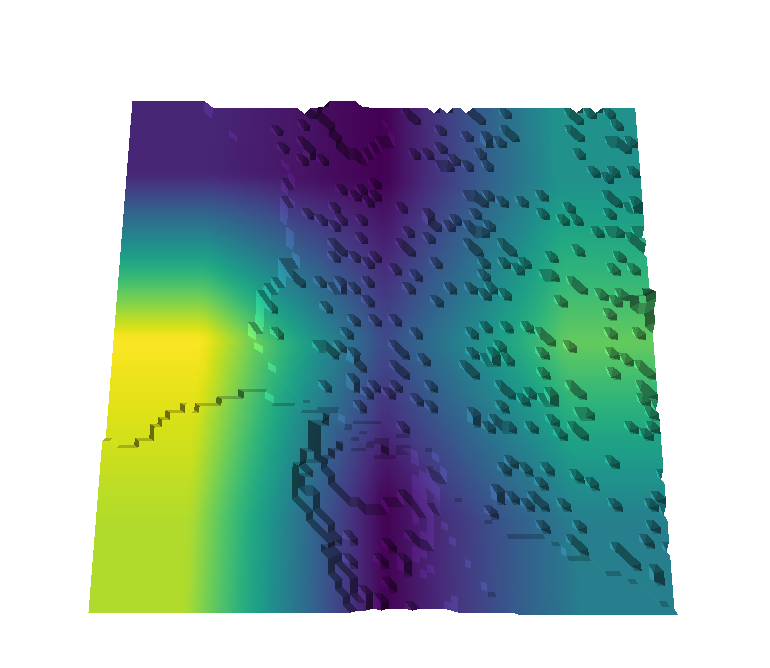
\includegraphics[width=\linewidth]{../img/5/quarry/best/20-patch-3d-majavi-colormap-0.png}
    \caption{0.20cm}
    \label{fig : quarry-best-1}
    \end{subfigure}
    \begin{subfigure}[b]{0.192\linewidth}
    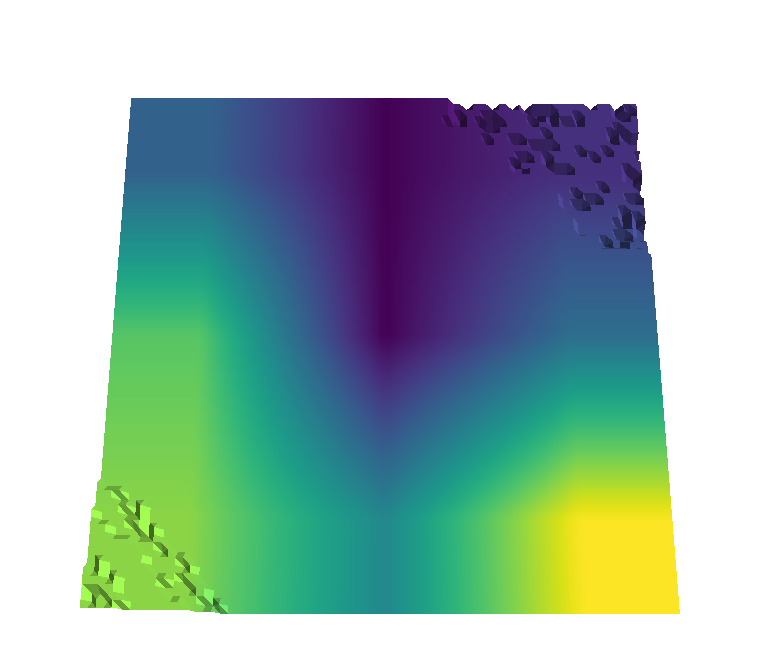
\includegraphics[width=\linewidth]{../img/5/quarry/best/25-patch-3d-majavi-colormap-10.png}
    \caption{0.26cm}
    \label{fig : quarry-best-2}
    \end{subfigure}
    \begin{subfigure}[b]{0.192\linewidth}
    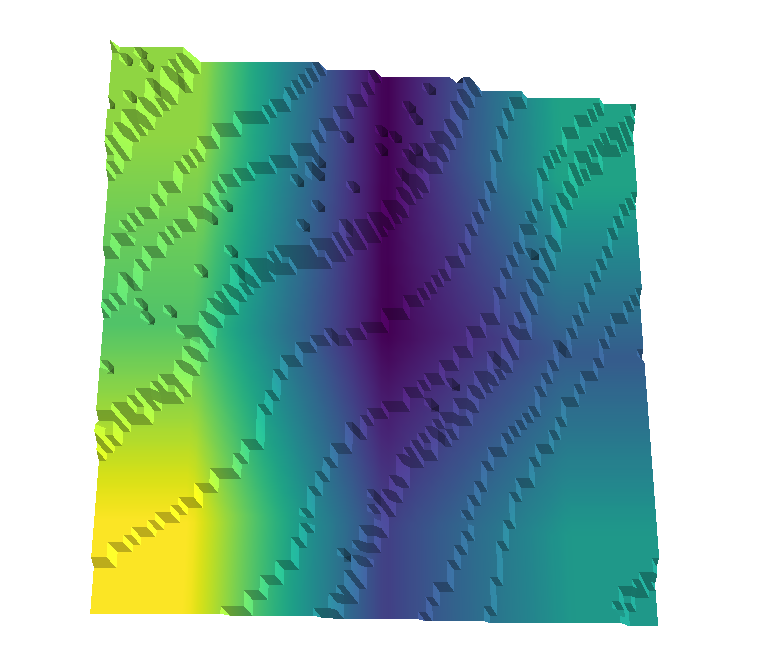
\includegraphics[width=\linewidth]{../img/5/quarry/best/30-patch-3d-majavi-colormap-20.png}
    \caption{0.30cm}
    \label{fig : quarry-best-3}
    \end{subfigure}
    \begin{subfigure}[b]{0.192\linewidth}
    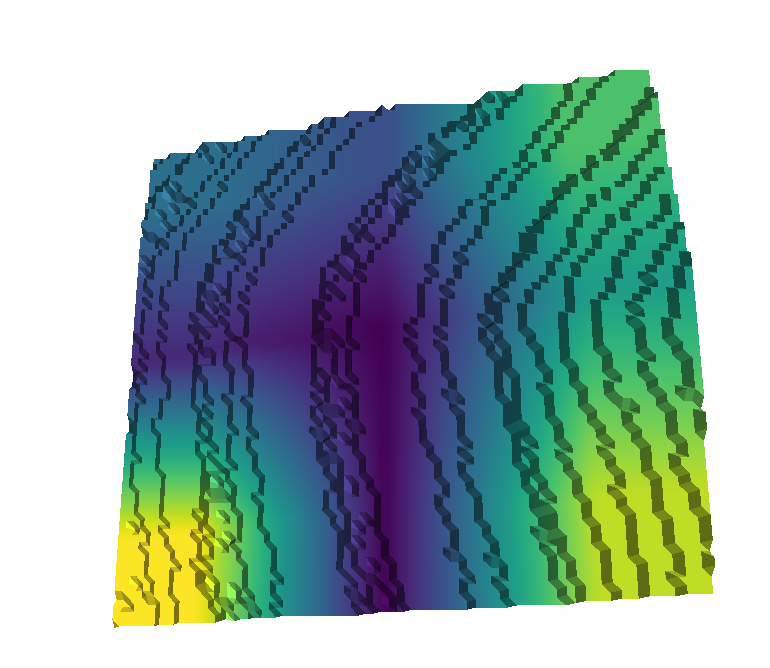
\includegraphics[width=\linewidth]{../img/5/quarry/best/34-patch-3d-majavi-colormap-30.png}
    \caption{0.35cm}
    \label{fig : quarry-best-4}
    \end{subfigure}
    \begin{subfigure}[b]{0.192\linewidth}
    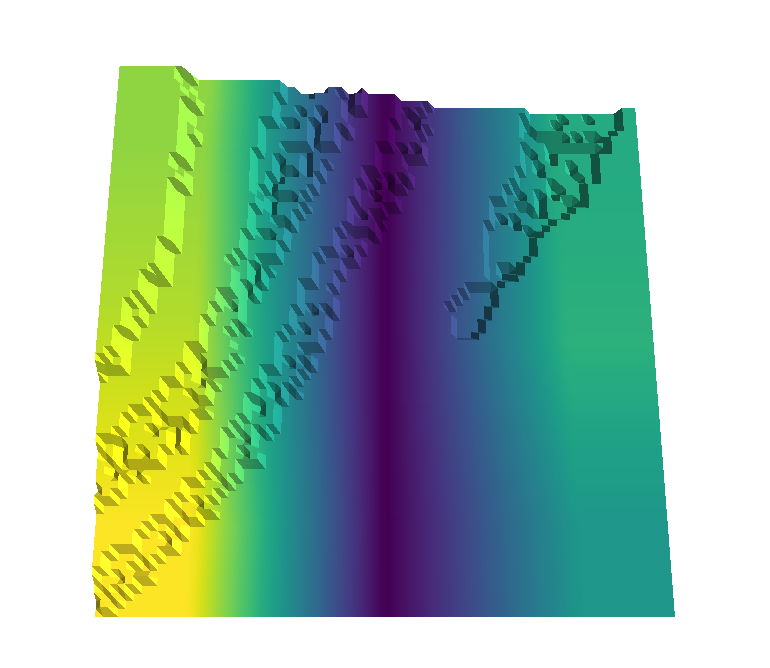
\includegraphics[width=\linewidth]{../img/5/quarry/best/38-patch-3d-majavi-colormap-40.png}
    \caption{0.38cm}
    \label{fig : quarry-best-5}
    \end{subfigure}
    \begin{subfigure}[b]{0.192\linewidth}
    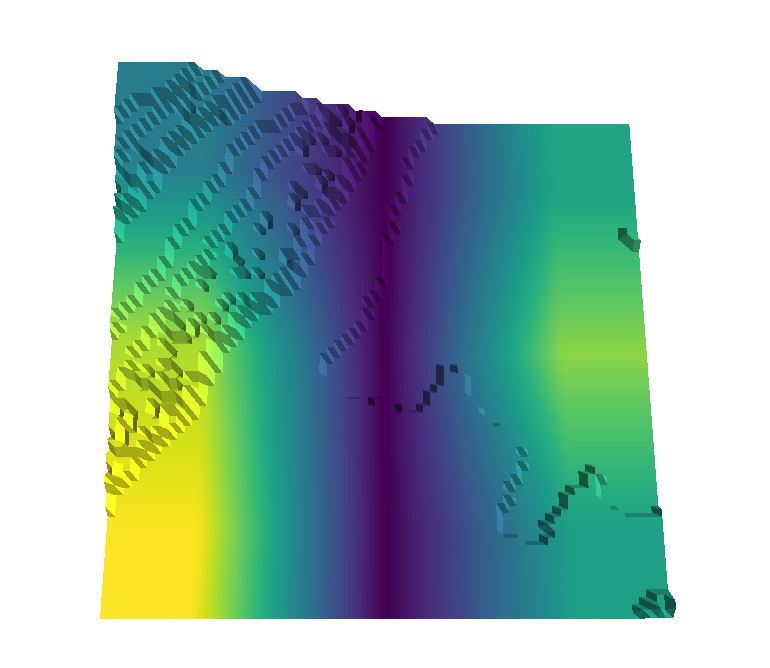
\includegraphics[width=\linewidth]{../img/5/quarry/best/41-patch-3d-majavi-colormap-50.png}
    \caption{0.41cm}
    \label{fig : quarry-best-6}
    \end{subfigure}
    \begin{subfigure}[b]{0.192\linewidth}
    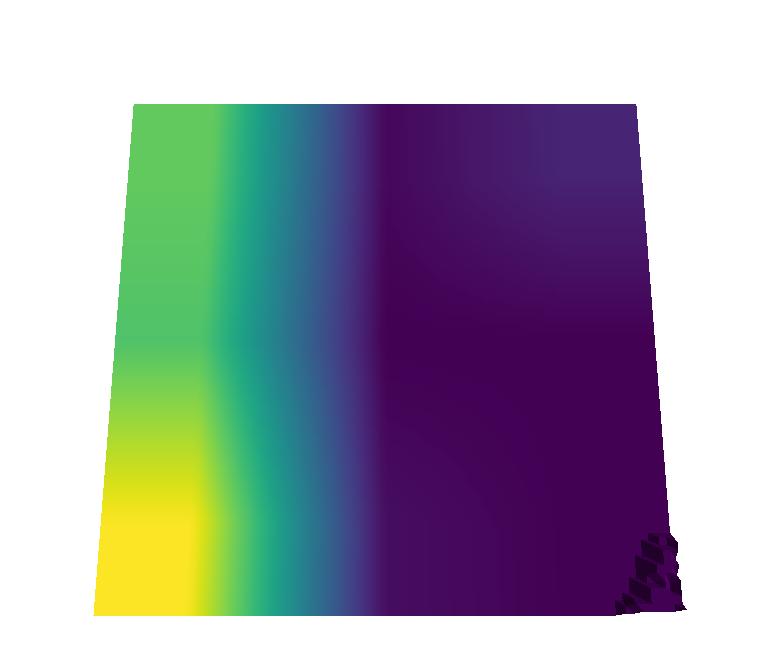
\includegraphics[width=\linewidth]{../img/5/quarry/best/44-patch-3d-majavi-colormap-60.png}
    \caption{0.44cm}
    \label{fig : quarry-best-7}
    \end{subfigure}
    \begin{subfigure}[b]{0.192\linewidth}
    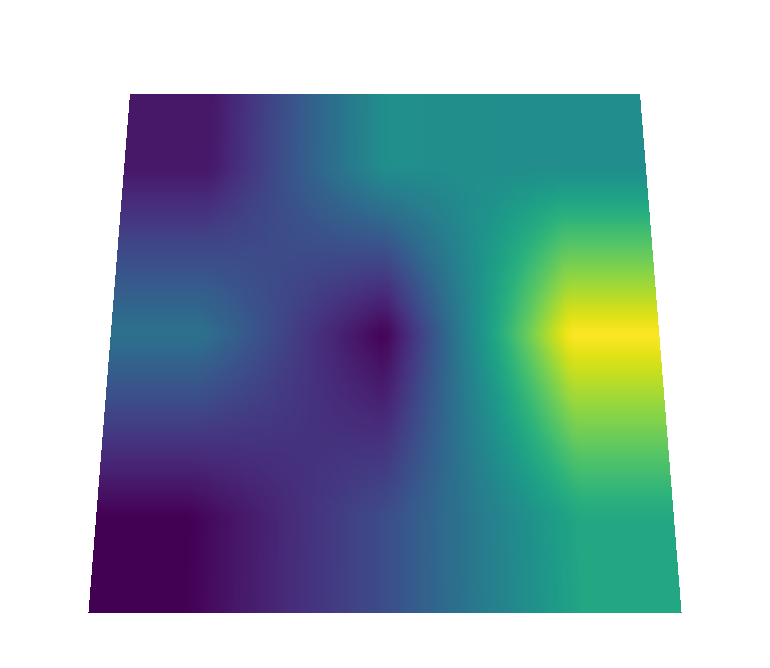
\includegraphics[width=\linewidth]{../img/5/quarry/best/46-patch-3d-majavi-colormap-70.png}
    \caption{0.47cm}
    \label{fig : quarry-best-8}
    \end{subfigure}
    \begin{subfigure}[b]{0.192\linewidth}
    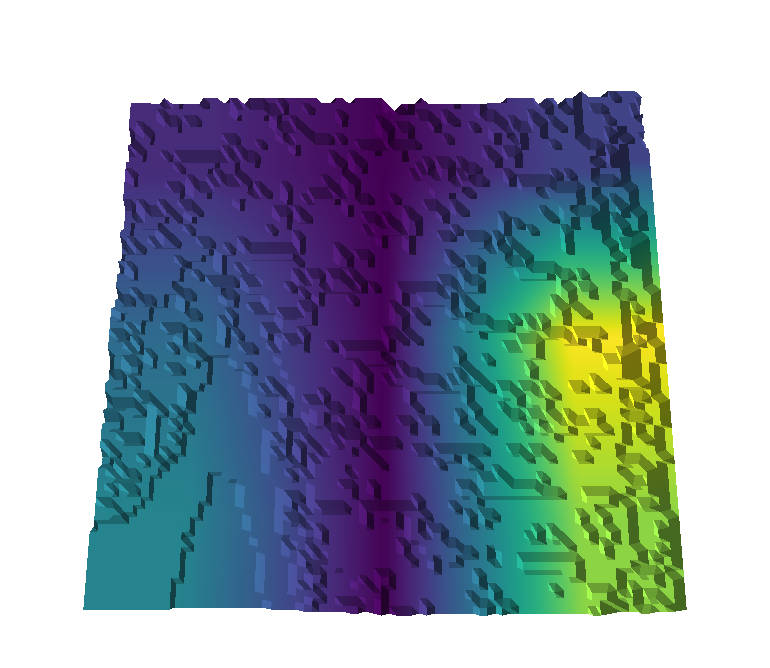
\includegraphics[width=\linewidth]{../img/5/quarry/best/49-patch-3d-majavi-colormap-80.png}
    \caption{0.49cm}
    \label{fig : quarry-best-9}
    \end{subfigure}
    \begin{subfigure}[b]{0.192\linewidth}
    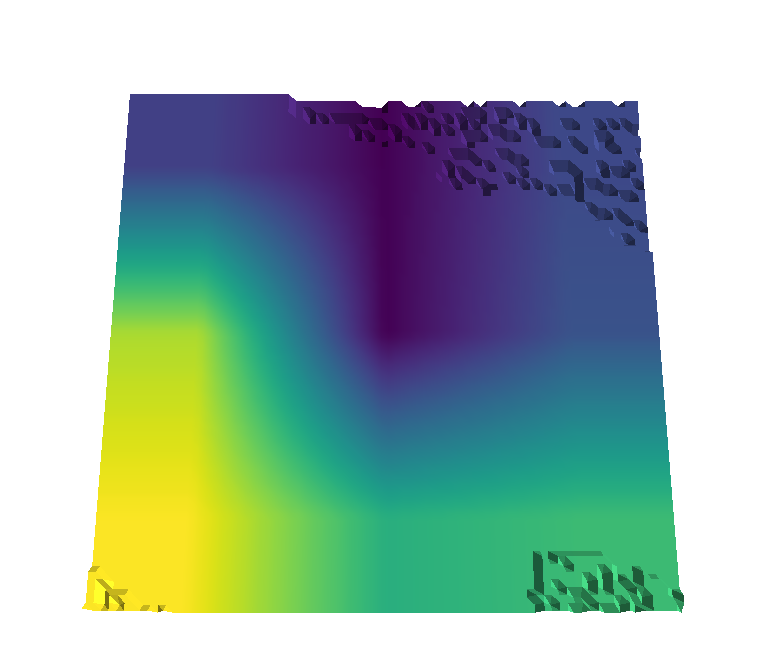
\includegraphics[width=\linewidth]{../img/5/quarry/best/51-patch-3d-majavi-colormap-90.png}
    \caption{0.52cm}
    \label{fig : quarry-best-10}
    \end{subfigure}
    \begin{subfigure}[b]{0.192\linewidth}
    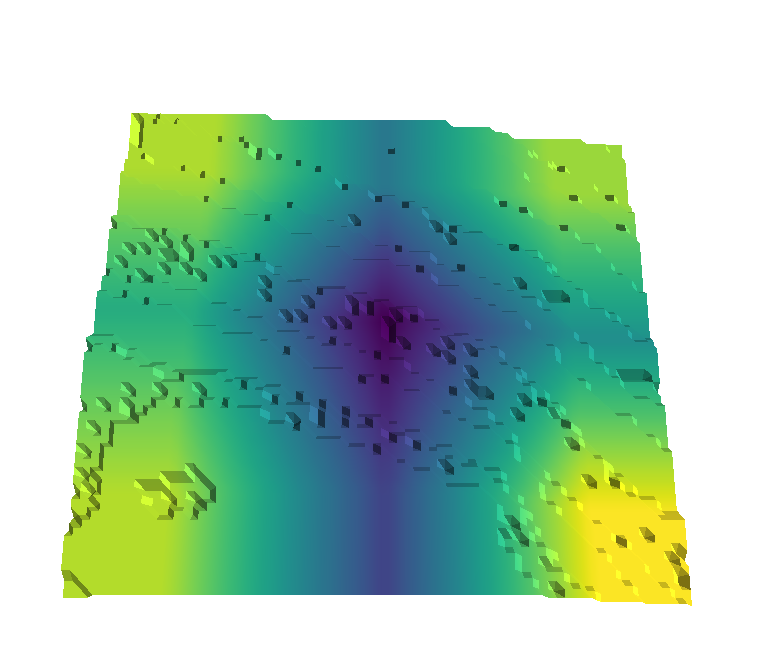
\includegraphics[width=\linewidth]{../img/5/quarry/best/54-patch-3d-majavi-colormap-100.png}
    \caption{0.54cm}
    \label{fig : quarry-best-11}
    \end{subfigure}
    \begin{subfigure}[b]{0.192\linewidth}
    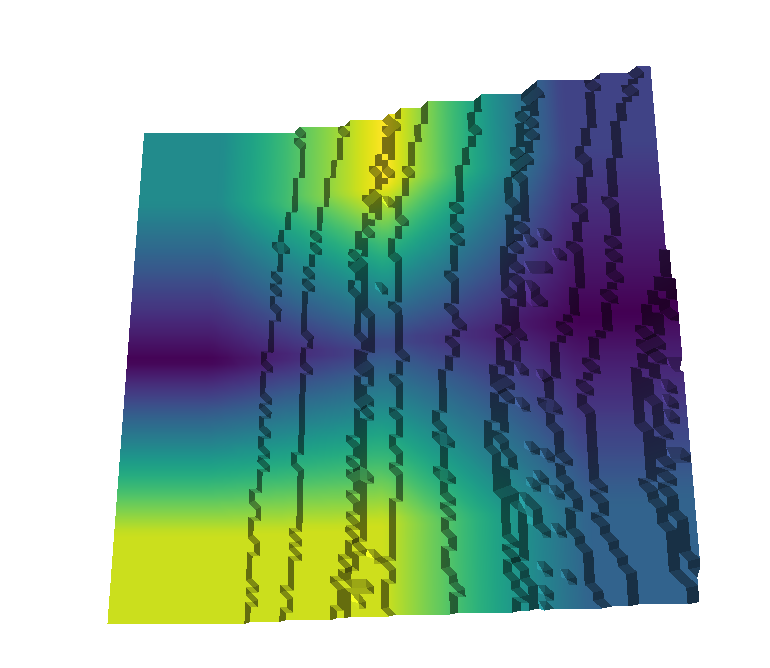
\includegraphics[width=\linewidth]{../img/5/quarry/best/56-patch-3d-majavi-colormap-110.png}
    \caption{0.57cm}
    \label{fig : quarry-best-12}
    \end{subfigure}
    \begin{subfigure}[b]{0.192\linewidth}
    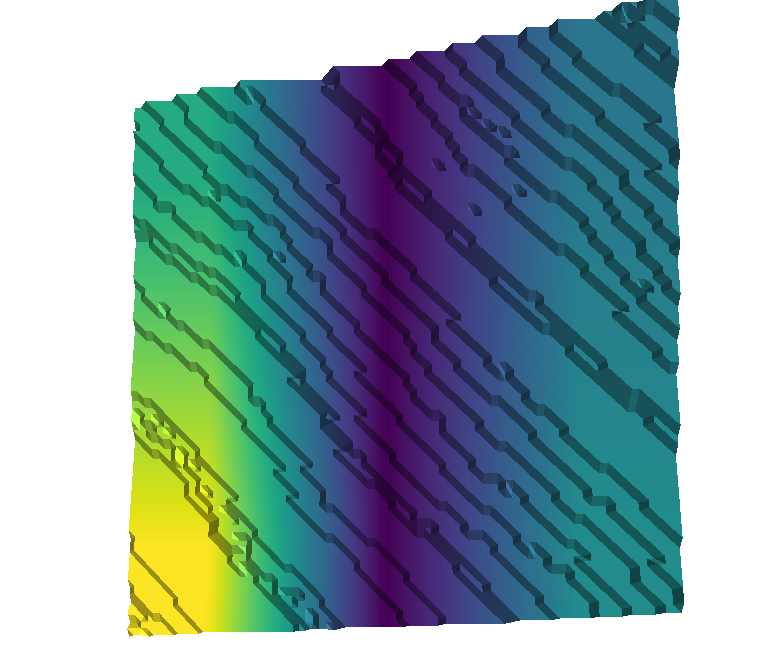
\includegraphics[width=\linewidth]{../img/5/quarry/best/58-patch-3d-majavi-colormap-120.png}
    \caption{0.59cm}
    \label{fig : quarry-best-13}
    \end{subfigure}
    \begin{subfigure}[b]{0.192\linewidth}
    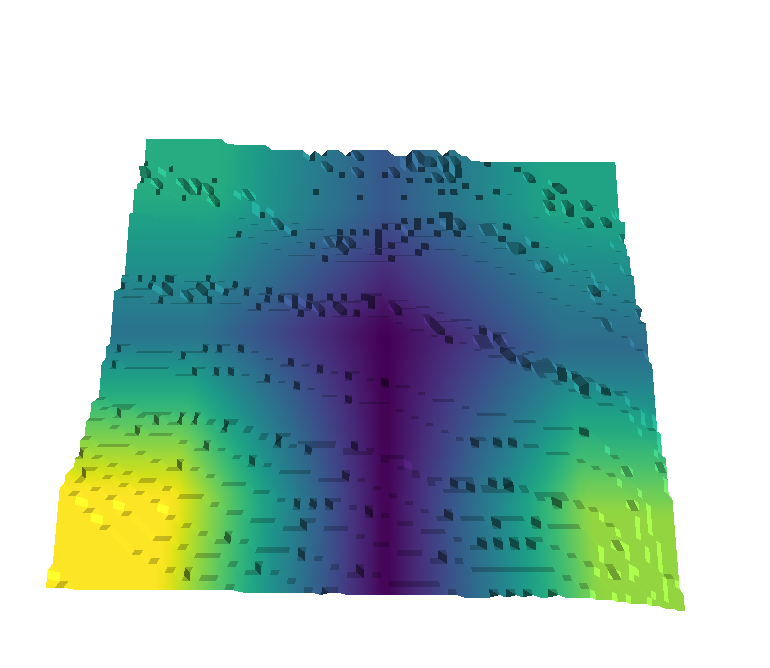
\includegraphics[width=\linewidth]{../img/5/quarry/best/60-patch-3d-majavi-colormap-130.png}
    \caption{0.60cm}
    \label{fig : quarry-best-14}
    \end{subfigure}
    \begin{subfigure}[b]{0.192\linewidth}
    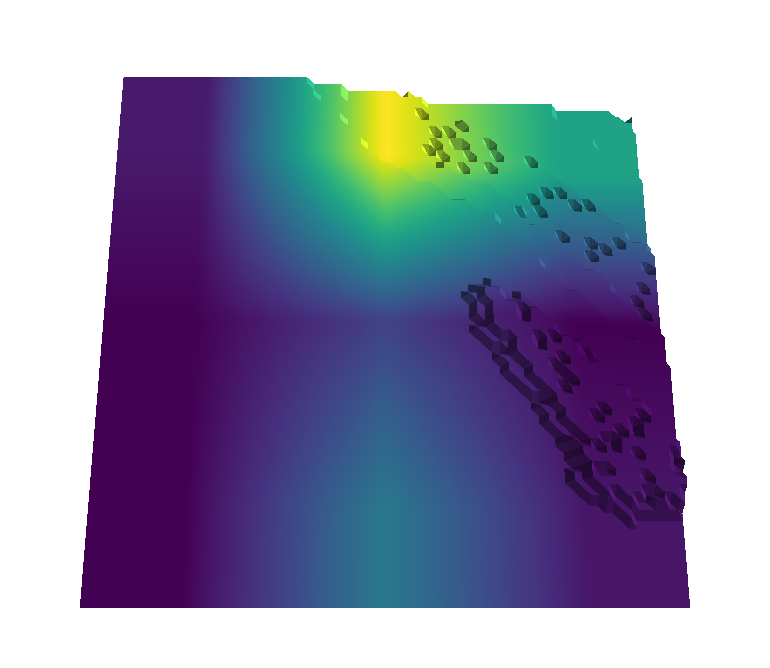
\includegraphics[width=\linewidth]{../img/5/quarry/best/62-patch-3d-majavi-colormap-140.png}
    \caption{0.62cm}
    \label{fig : quarry-best-15}
    \end{subfigure}
    \begin{subfigure}[b]{0.192\linewidth}
    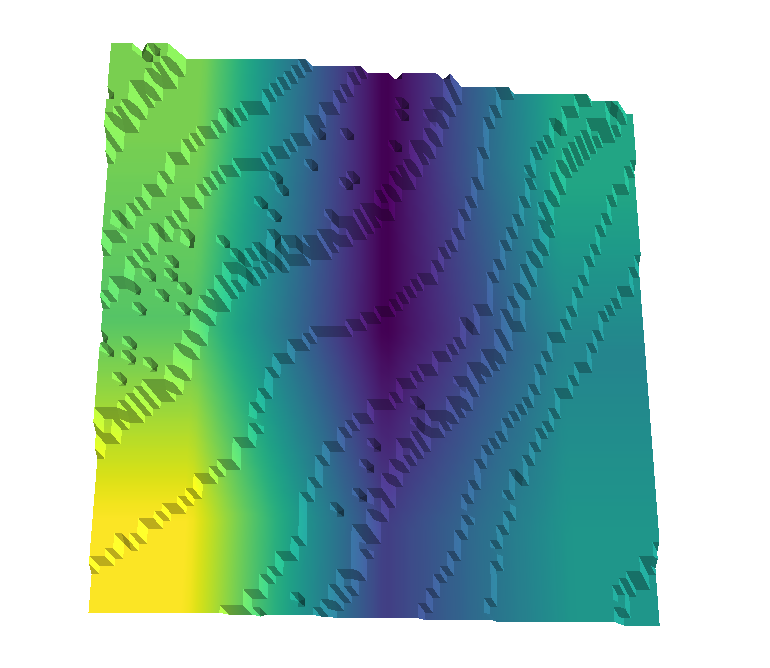
\includegraphics[width=\linewidth]{../img/5/quarry/best/63-patch-3d-majavi-colormap-150.png}
    \caption{0.64cm}
    \label{fig : quarry-best-16}
    \end{subfigure}
    \begin{subfigure}[b]{0.192\linewidth}
    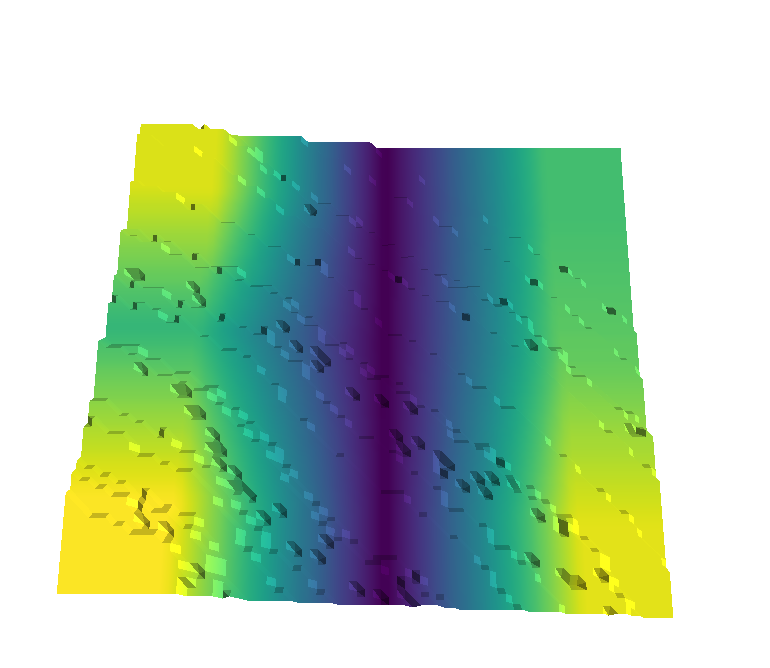
\includegraphics[width=\linewidth]{../img/5/quarry/best/65-patch-3d-majavi-colormap-160.png}
    \caption{0.66cm}
    \label{fig : quarry-best-17}
    \end{subfigure}
    \begin{subfigure}[b]{0.192\linewidth}
    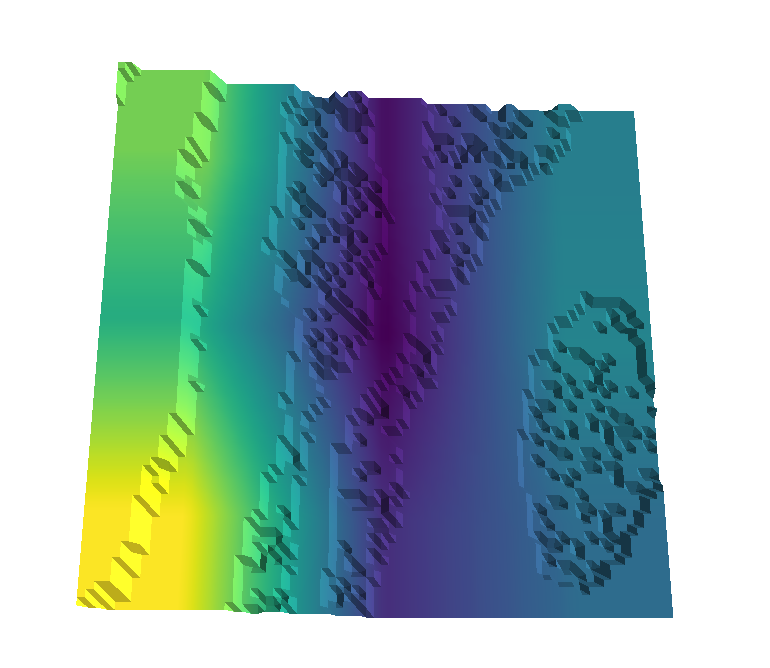
\includegraphics[width=\linewidth]{../img/5/quarry/best/67-patch-3d-majavi-colormap-170.png}
    \caption{0.67cm}
    \label{fig : quarry-best-18}
    \end{subfigure}
    \begin{subfigure}[b]{0.192\linewidth}
    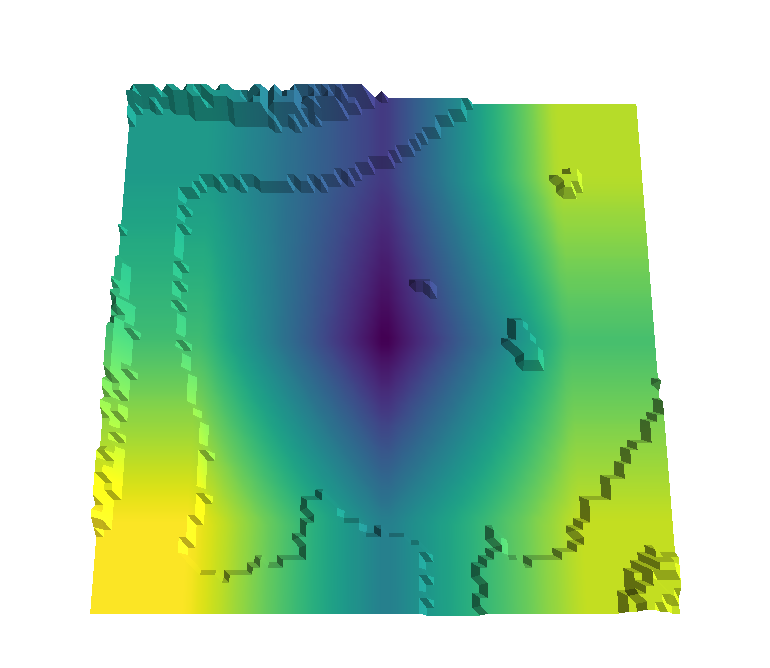
\includegraphics[width=\linewidth]{../img/5/quarry/best/68-patch-3d-majavi-colormap-180.png}
    \caption{0.68cm}
    \label{fig : quarry-best-19}
    \end{subfigure}
    \begin{subfigure}[b]{0.192\linewidth}
    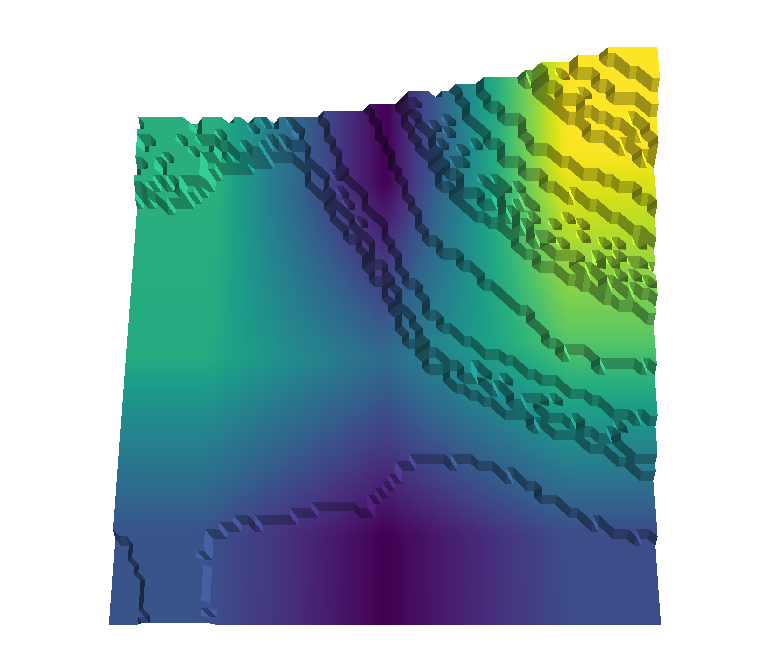
\includegraphics[width=\linewidth]{../img/5/quarry/best/70-patch-3d-majavi-colormap-190.png}
    \caption{0.70cm}
    \label{fig : quarry-best-20}
    \end{subfigure}
    \label{fig : quarry-best}
    \caption{Traversable patches sampled from the test dataset correctly predicted by the model. We compute dthe Grad-CAM and applied as texture in the 3D render. The yellow highlights the ground region that contributed the most the model's prediction. }
    \end{figure}

\subsection{Non traversable patches}
    Not traversable patches correctly classified by the model. In this case, the region highlighted by the Grad-CAM more varied. Like in the previous section, in some patches, \ref{fig : quarry-worst-2}, \ref{fig : quarry-worst-6}, \ref{fig : quarry-worst-12}, \ref{fig : quarry-worst-14}, \ref{fig : quarry-worst-17}, \ref{fig : quarry-worst-19}, the non traversable features is directly under the robot. While, on other grounds with a atraversable left part but a big obstacle ahead, figures \ref{fig : quarry-worst-3}, \ref{fig : quarry-worst-5}, \ref{fig : quarry-worst-9}, \ref{fig : quarry-worst-15}, \ref{fig : quarry-worst-18}, the model identified the huge obstacle as the main reason for their untraversability. There mixed cases, figures \ref{fig : quarry-worst-2}, \ref{fig : quarry-worst-4}, \ref{fig : quarry-worst-10}, \ref{fig : quarry-worst-13}. Other grounds are mostly uneven, \ref{fig : quarry-worst-4}, \ref{fig : quarry-worst-11} and \ref{fig : quarry-worst-12} and the cam highlighted the biggest bumps. The last patch, \ref{fig : quarry-worst-8}, is very interesting. There is a trail with a obstacle parallel to it. Perfectly, the network identified one part obstacle as responsabile for the prediction. Probably, these spot is the points where the robot hitted the obstacle while going forward.

    \begin{figure}[H]
        \centering
        \begin{subfigure}[b]{0.192\linewidth}
        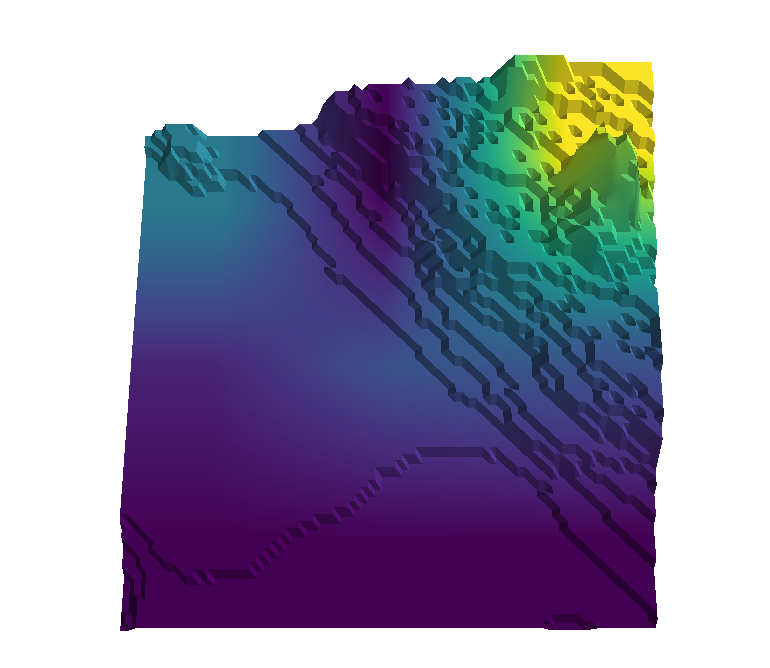
\includegraphics[width=\linewidth]{../img/5/quarry/worst/-35-patch-3d-majavi-colormap-0.png}
        \caption{-0.36cm}
        \label{fig : quarry-worst-1}
        \end{subfigure}
        \begin{subfigure}[b]{0.192\linewidth}
        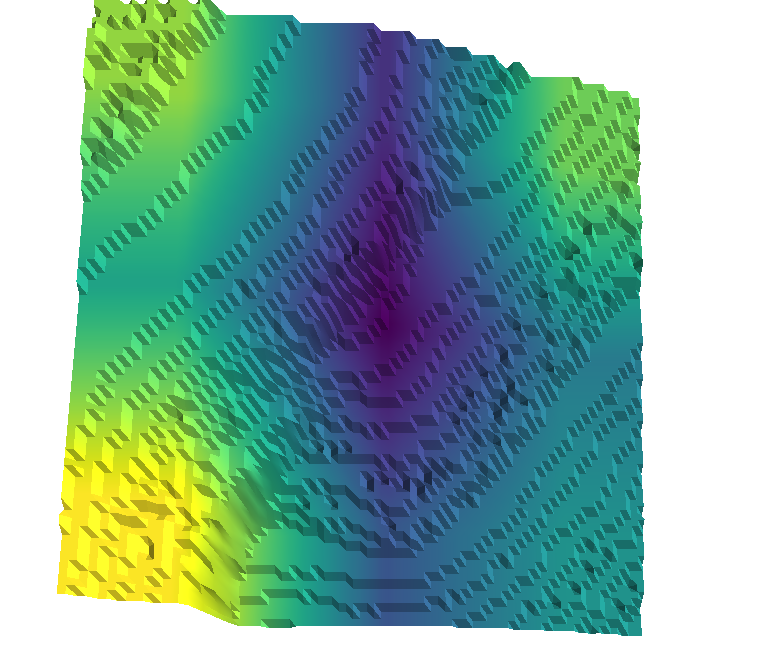
\includegraphics[width=\linewidth]{../img/5/quarry/worst/-7-patch-3d-majavi-colormap-10.png}
        \caption{-0.08cm}
        \label{fig : quarry-worst-2}
        \end{subfigure}
        \begin{subfigure}[b]{0.192\linewidth}
        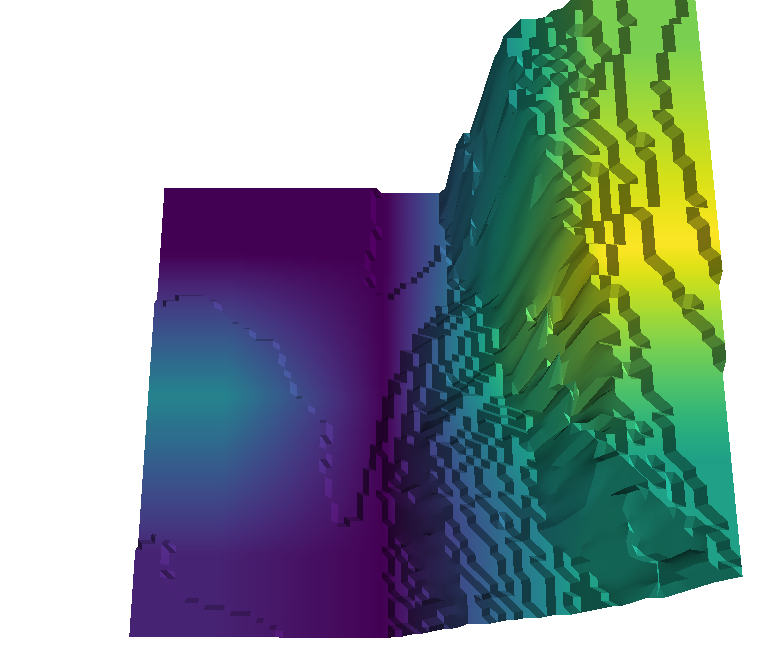
\includegraphics[width=\linewidth]{../img/5/quarry/worst/-4-patch-3d-majavi-colormap-20.png}
        \caption{-0.05cm}
        \label{fig : quarry-worst-3}
        \end{subfigure}
        \begin{subfigure}[b]{0.192\linewidth}
        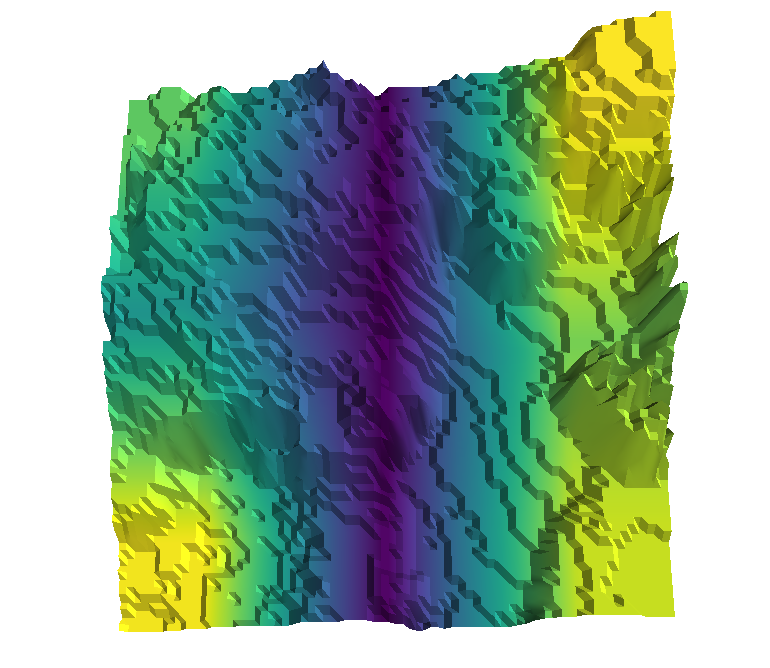
\includegraphics[width=\linewidth]{../img/5/quarry/worst/-3-patch-3d-majavi-colormap-30.png}
        \caption{-0.03cm}
        \label{fig : quarry-worst-4}
        \end{subfigure}
        \begin{subfigure}[b]{0.192\linewidth}
        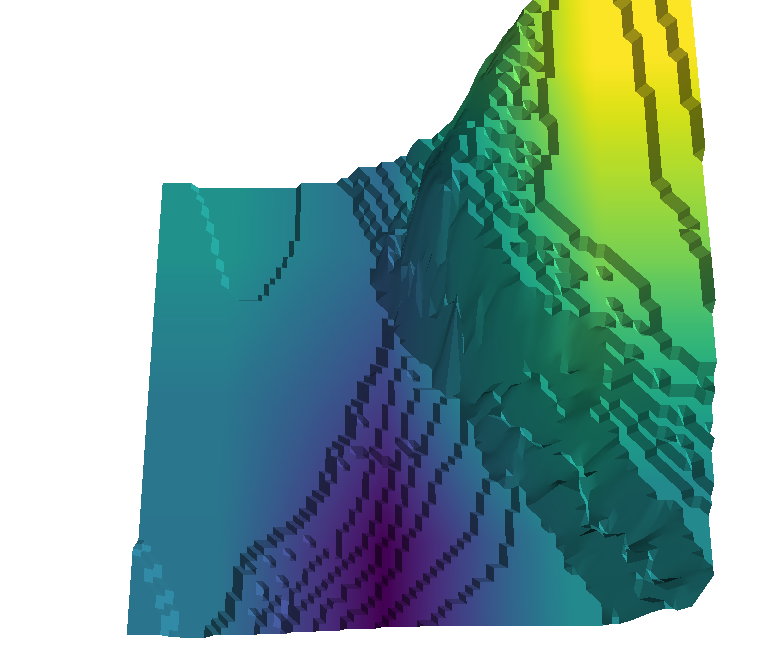
\includegraphics[width=\linewidth]{../img/5/quarry/worst/-2-patch-3d-majavi-colormap-40.png}
        \caption{-0.02cm}
        \label{fig : quarry-worst-5}
        \end{subfigure}
        \begin{subfigure}[b]{0.192\linewidth}
        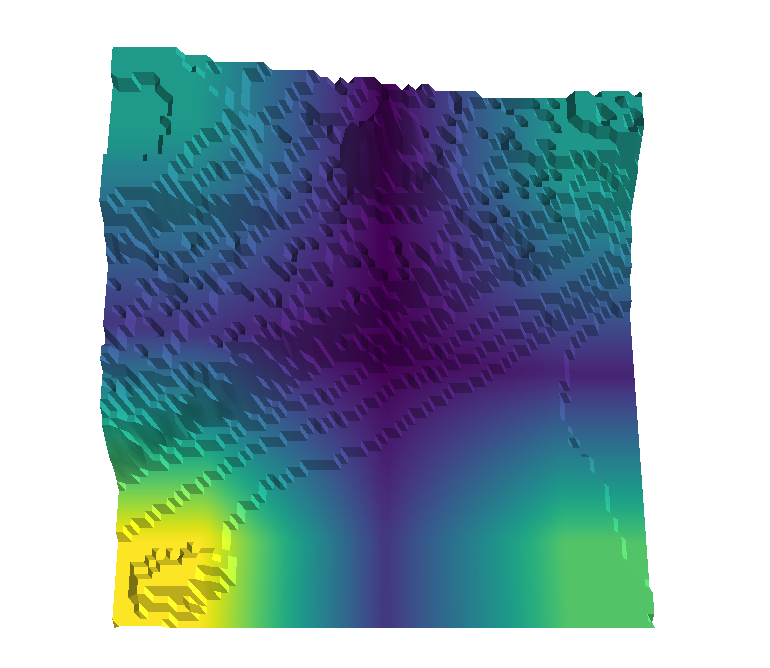
\includegraphics[width=\linewidth]{../img/5/quarry/worst/-1-patch-3d-majavi-colormap-50.png}
        \caption{-0.01cm}
        \label{fig : quarry-worst-6}
        \end{subfigure}
        \begin{subfigure}[b]{0.192\linewidth}
        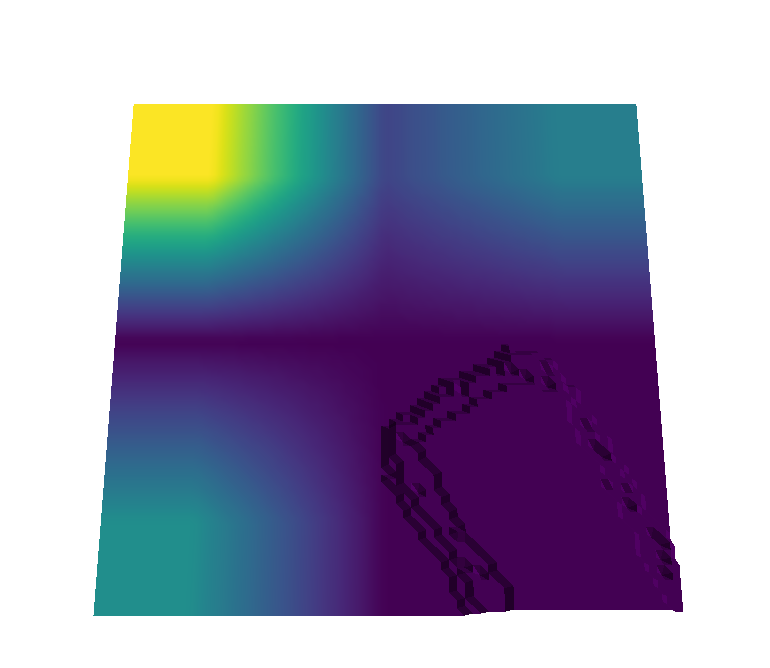
\includegraphics[width=\linewidth]{../img/5/quarry/worst/00-patch-3d-majavi-colormap-60.png}
        \caption{-0.01cm}
        \label{fig : quarry-worst-7}
        \end{subfigure}
        \begin{subfigure}[b]{0.192\linewidth}
        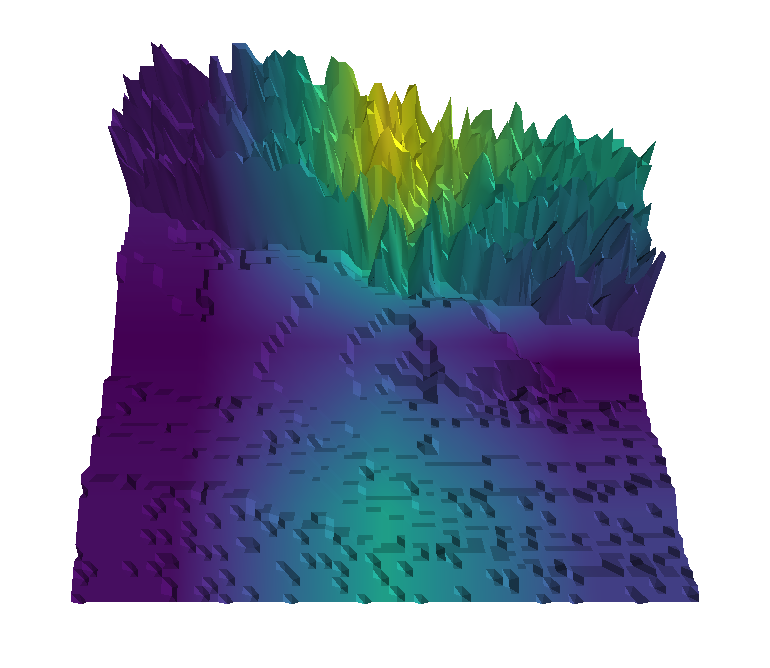
\includegraphics[width=\linewidth]{../img/5/quarry/worst/00-patch-3d-majavi-colormap-70.png}
        \caption{0.00cm}
        \label{fig : quarry-worst-8}
        \end{subfigure}
        \begin{subfigure}[b]{0.192\linewidth}
        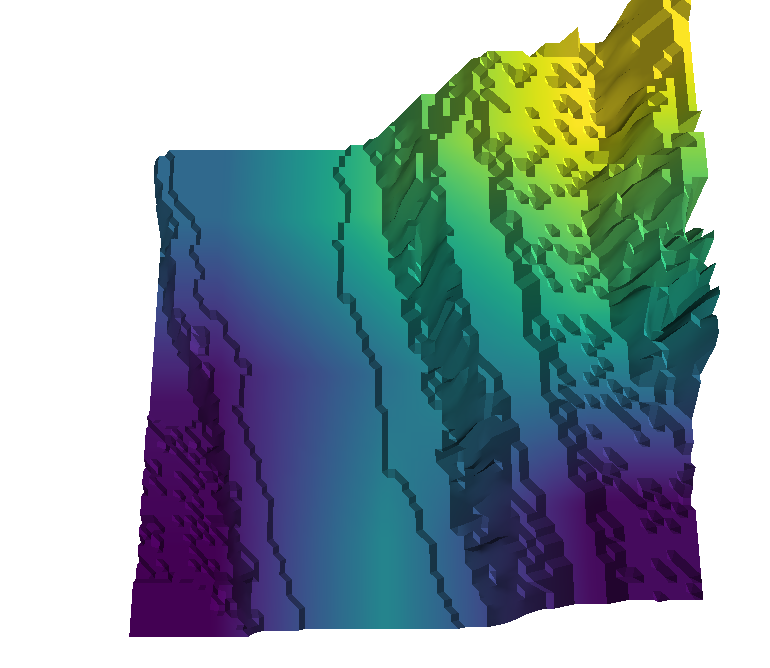
\includegraphics[width=\linewidth]{../img/5/quarry/worst/00-patch-3d-majavi-colormap-80.png}
        \caption{0.01cm}
        \label{fig : quarry-worst-9}
        \end{subfigure}
        \begin{subfigure}[b]{0.192\linewidth}
        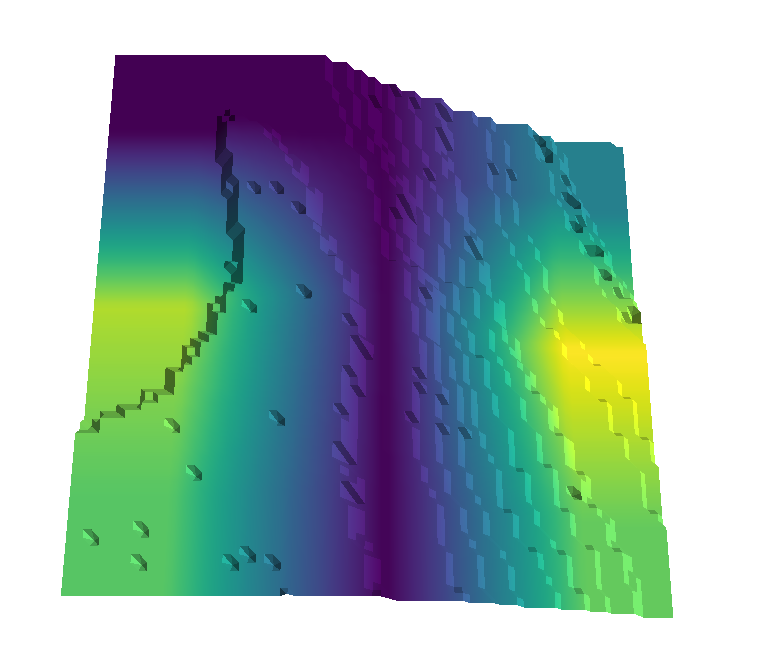
\includegraphics[width=\linewidth]{../img/5/quarry/worst/01-patch-3d-majavi-colormap-90.png}
        \caption{0.02cm}
        \label{fig : quarry-worst-10}
        \end{subfigure}
        \begin{subfigure}[b]{0.192\linewidth}
        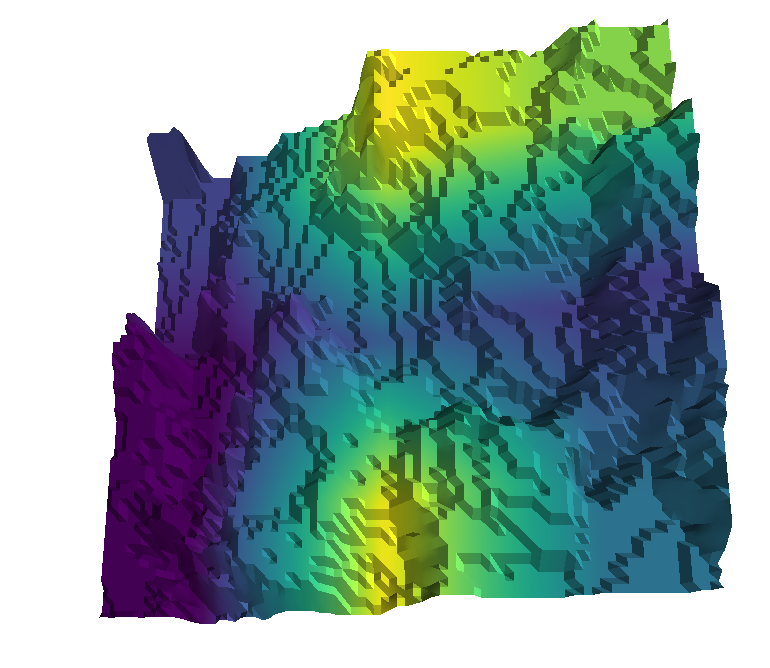
\includegraphics[width=\linewidth]{../img/5/quarry/worst/02-patch-3d-majavi-colormap-100.png}
        \caption{0.02cm}
        \label{fig : quarry-worst-11}
        \end{subfigure}
        \begin{subfigure}[b]{0.192\linewidth}
        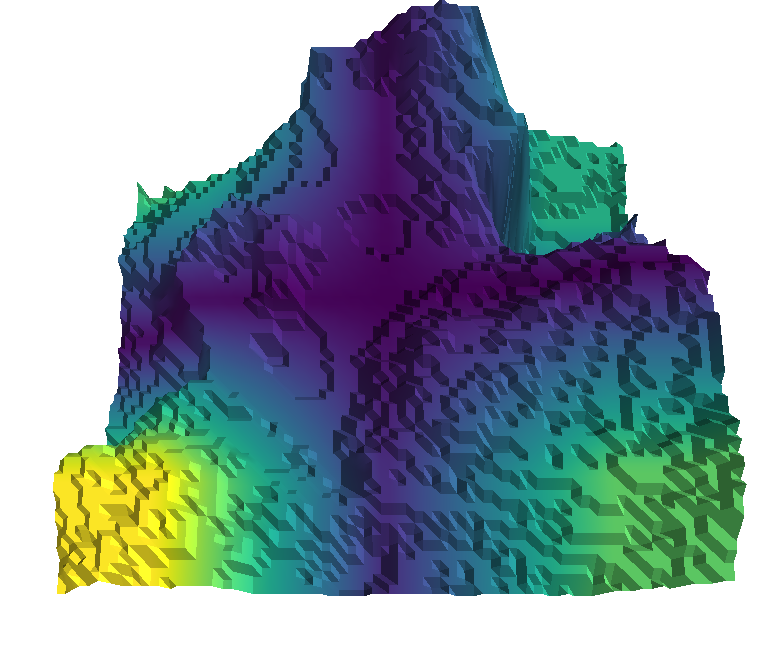
\includegraphics[width=\linewidth]{../img/5/quarry/worst/03-patch-3d-majavi-colormap-110.png}
        \caption{0.03cm}
        \label{fig : quarry-worst-12}
        \end{subfigure}
        \begin{subfigure}[b]{0.192\linewidth}
        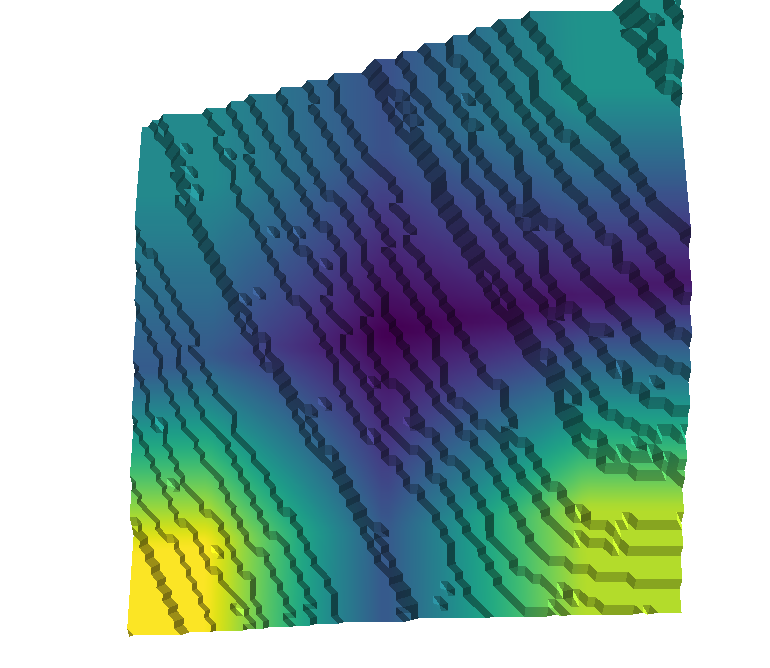
\includegraphics[width=\linewidth]{../img/5/quarry/worst/04-patch-3d-majavi-colormap-120.png}
        \caption{0.05cm}
        \label{fig : quarry-worst-13}
        \end{subfigure}
        \begin{subfigure}[b]{0.192\linewidth}
        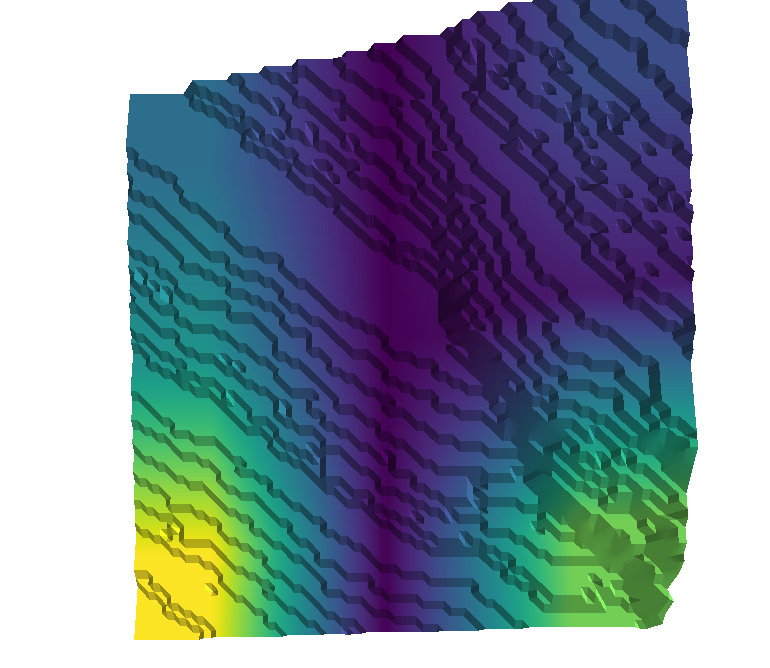
\includegraphics[width=\linewidth]{../img/5/quarry/worst/06-patch-3d-majavi-colormap-130.png}
        \caption{0.06cm}
        \label{fig : quarry-worst-14}
        \end{subfigure}
        \begin{subfigure}[b]{0.192\linewidth}
        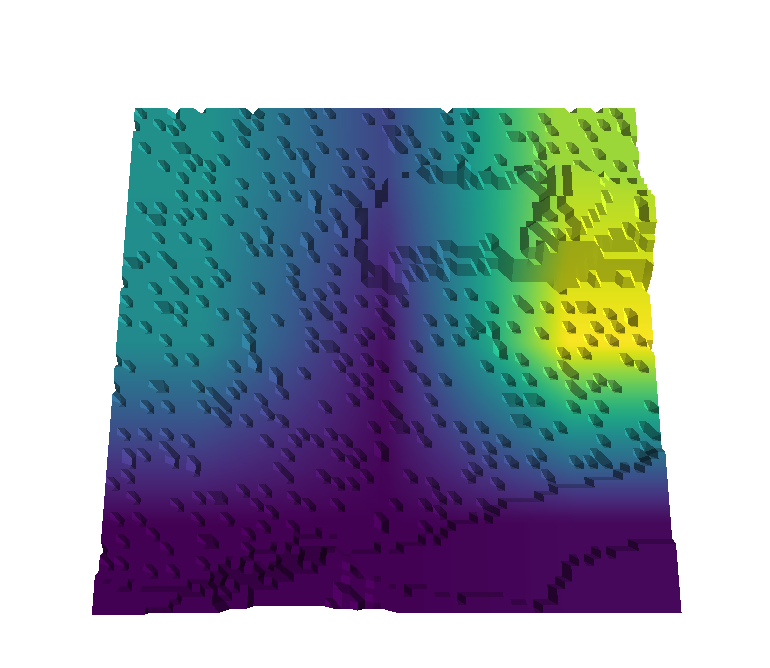
\includegraphics[width=\linewidth]{../img/5/quarry/worst/07-patch-3d-majavi-colormap-140.png}
        \caption{0.08cm}
        \label{fig : quarry-worst-15}
        \end{subfigure}
        \begin{subfigure}[b]{0.192\linewidth}
        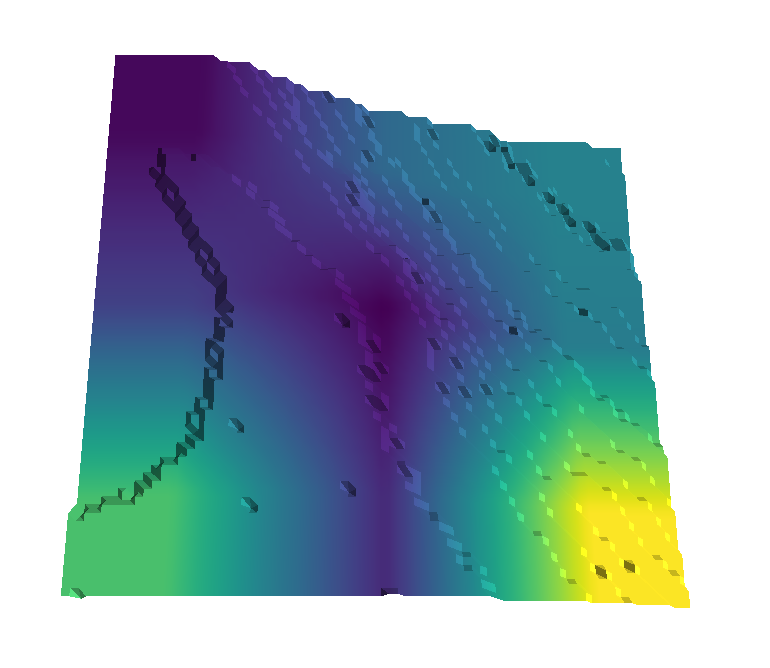
\includegraphics[width=\linewidth]{../img/5/quarry/worst/09-patch-3d-majavi-colormap-150.png}
        \caption{0.10cm}
        \label{fig : quarry-worst-16}
        \end{subfigure}
        \begin{subfigure}[b]{0.192\linewidth}
        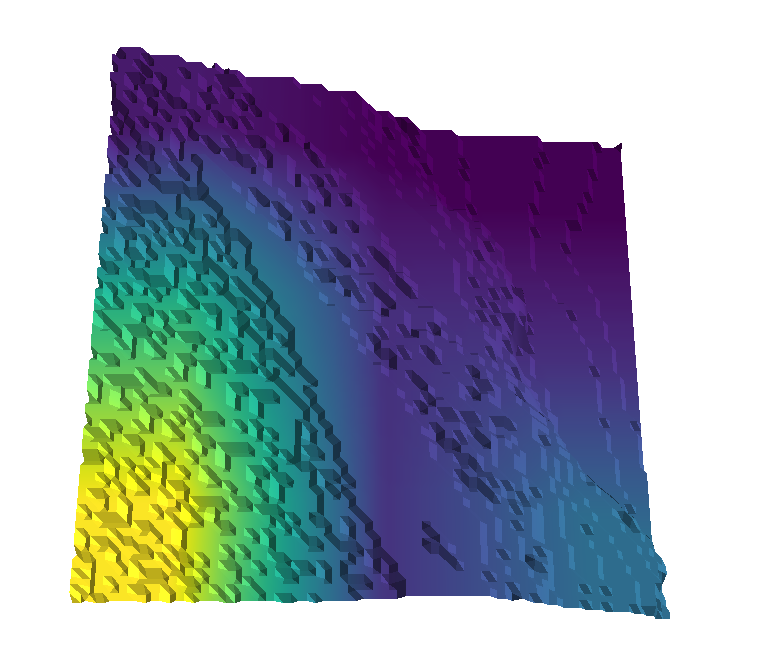
\includegraphics[width=\linewidth]{../img/5/quarry/worst/11-patch-3d-majavi-colormap-160.png}
        \caption{0.11cm}
        \label{fig : quarry-worst-17}
        \end{subfigure}
        \begin{subfigure}[b]{0.192\linewidth}
        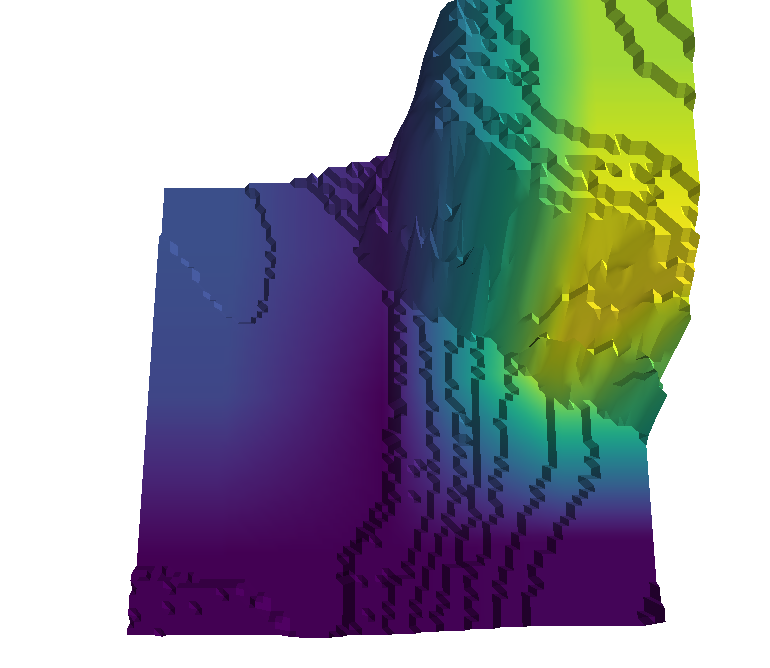
\includegraphics[width=\linewidth]{../img/5/quarry/worst/13-patch-3d-majavi-colormap-170.png}
        \caption{0.13cm}
        \label{fig : quarry-worst-18}
        \end{subfigure}
        \begin{subfigure}[b]{0.192\linewidth}
        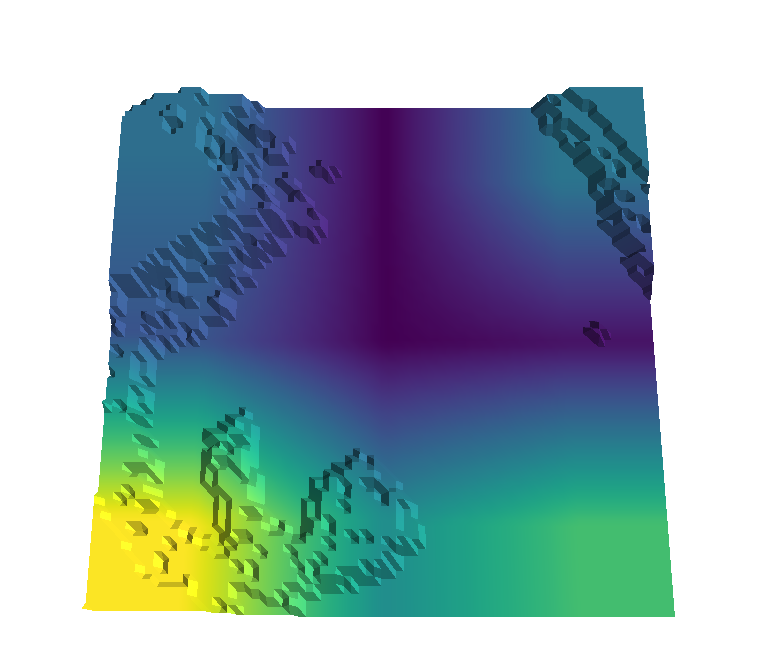
\includegraphics[width=\linewidth]{../img/5/quarry/worst/15-patch-3d-majavi-colormap-180.png}
        \caption{0.15cm}
        \label{fig : quarry-worst-19}
        \end{subfigure}
        \begin{subfigure}[b]{0.192\linewidth}
        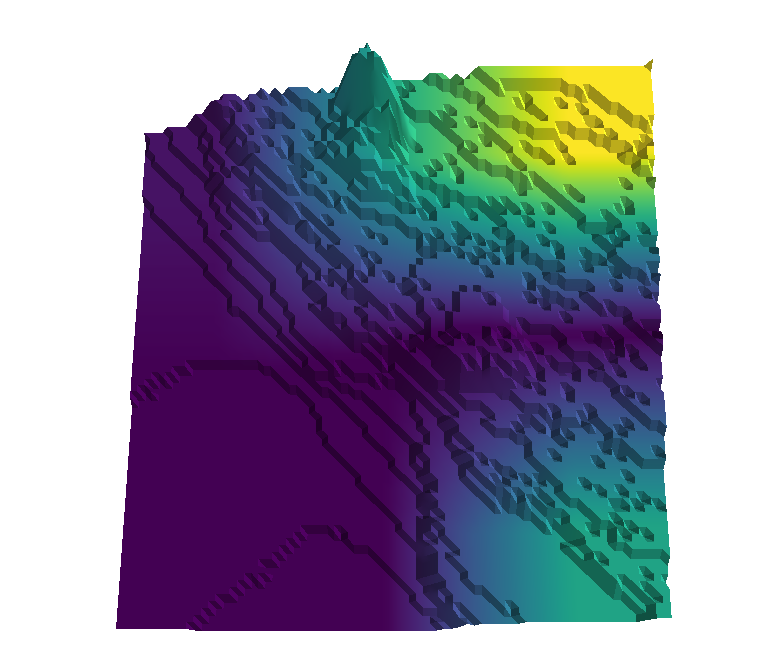
\includegraphics[width=\linewidth]{../img/5/quarry/worst/17-patch-3d-majavi-colormap-190.png}
        \caption{0.17cm}
        \label{fig : quarry-worst-20}
        \end{subfigure}
        \caption{Not traversable patches sampled from the test dataset correctly predicted by the model. We compute dthe Grad-CAM and applied as texture in the 3D render. The yellow highlights the ground region that contributed the most the model's prediction. }
        \label{fig : quarry-worst}
        \end{figure}
\subsection{False negative patches}
Not traversable inputs predicted as traversable by the model. Some of the grounds are similar to ones from the last section. Figure \ref{fig : quarry-worst-2} is almost identical to \ref{fig : quarry-false_negative-4}. In this case, the model must have misclassified the first part of the map thinking it could traverse till the two bumps in the end. If so, the robot should have been able to move for more than twenty centimeters. There are two grounds with a trail, \ref{fig : quarry-false_negative-14}, \ref{fig : quarry-false_negative-20}. In both cases, the model looked at the initial position of the robot, left, and the final part of the patch to understand if the robot fits on the trail. Moreover, there are different slopes in which Grad-CAM highlighted the region under the robot,  \ref{fig : quarry-false_negative-3},  \ref{fig : quarry-false_negative-4},  \ref{fig : quarry-false_negative-5},  \ref{fig : quarry-false_negative-7},  \ref{fig : quarry-false_negative-8},  \ref{fig : quarry-false_negative-19}. These regions may be hard to estimate when the sizes of the obstacles are closes to the edge cases. The model may overestimate when the size of the obstacle is just a few centimeters more than the real traversable one. Figure \ref{fig : quarry-false_negative-11} has a small step on the right region, correctly highlighted by Grad-CAM. Other patches have obstacles close to the end, \ref{fig : quarry-false_negative-10}, \ref{fig : quarry-false_negative-15}, \ref{fig : quarry-false_negative-16}, \ref{fig : quarry-false_negative-17}, \ref{fig : quarry-false_negative-18}. ONe patch clearly showed the model confusion, figure \ref{fig : quarry-false_negative-13}. Even if the obstacle was ahead, the model discriminated and an empty spot on the top left. 
in general, most of the region of interested on these patches are located on the left, close to the position of the robot's leg. Correctly, even if the prediction is wrong, the model looks at the first region of the surface, located near the legs, that can effect traversability. This shows the correct behavior even when misclassifying the inputs, meaning that the network is always looking in the correct spot. 
\begin{figure}[H]
    \centering
    \begin{subfigure}[b]{0.192\linewidth}
    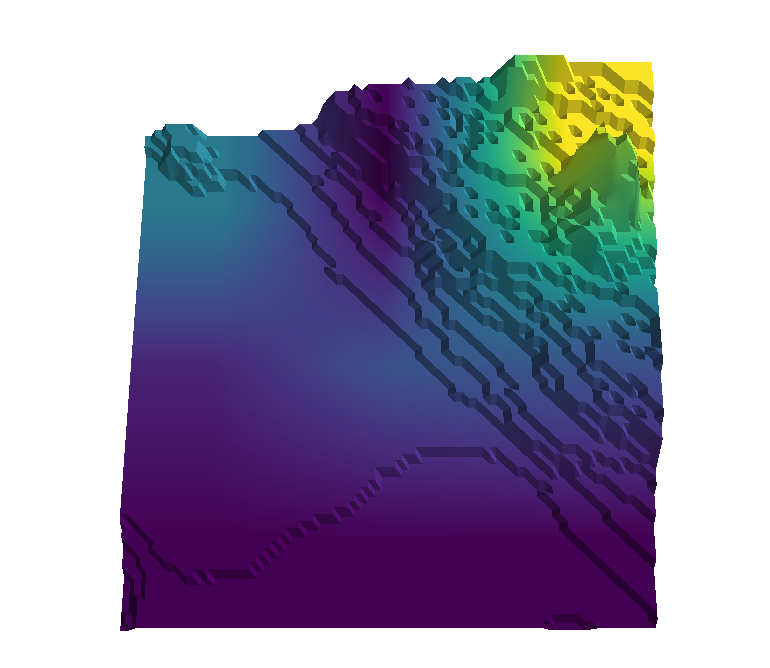
\includegraphics[width=\linewidth]{../img/5/quarry/false_negative/-14-patch-3d-majavi-colormap-0.png}
    \caption{-0.14cm}
    \label{fig : quarry-false_negative-1}
    \end{subfigure}
    \begin{subfigure}[b]{0.192\linewidth}
    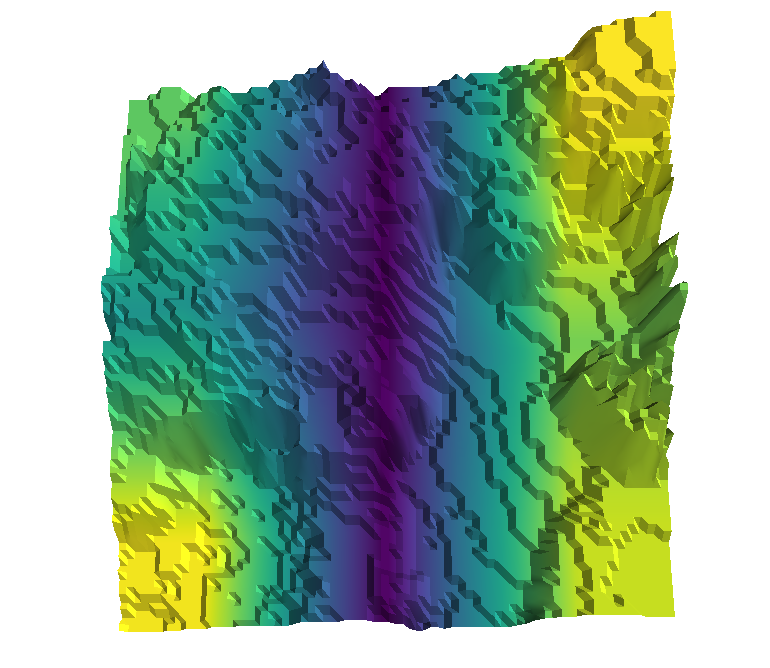
\includegraphics[width=\linewidth]{../img/5/quarry/false_negative/-6-patch-3d-majavi-colormap-10.png}
    \caption{-0.07cm}
    \label{fig : quarry-false_negative-2}
    \end{subfigure}
    \begin{subfigure}[b]{0.192\linewidth}
    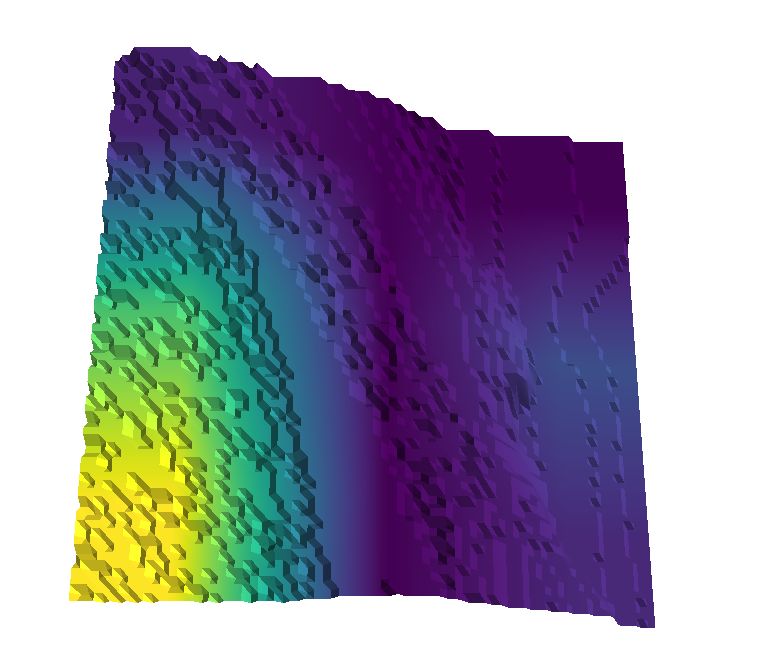
\includegraphics[width=\linewidth]{../img/5/quarry/false_negative/-4-patch-3d-majavi-colormap-20.png}
    \caption{-0.05cm}
    \label{fig : quarry-false_negative-3}
    \end{subfigure}
    \begin{subfigure}[b]{0.192\linewidth}
    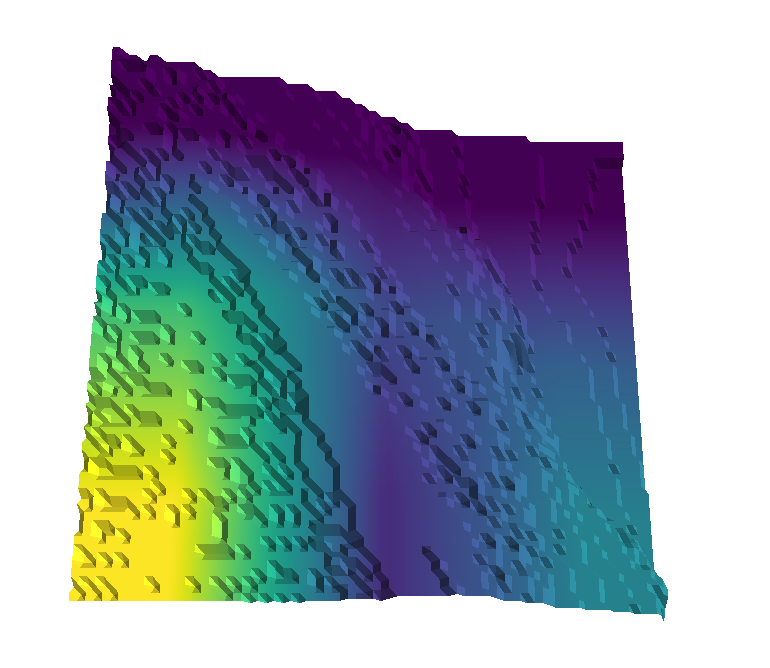
\includegraphics[width=\linewidth]{../img/5/quarry/false_negative/-2-patch-3d-majavi-colormap-30.png}
    \caption{-0.02cm}
    \label{fig : quarry-false_negative-4}
    \end{subfigure}
    \begin{subfigure}[b]{0.192\linewidth}
    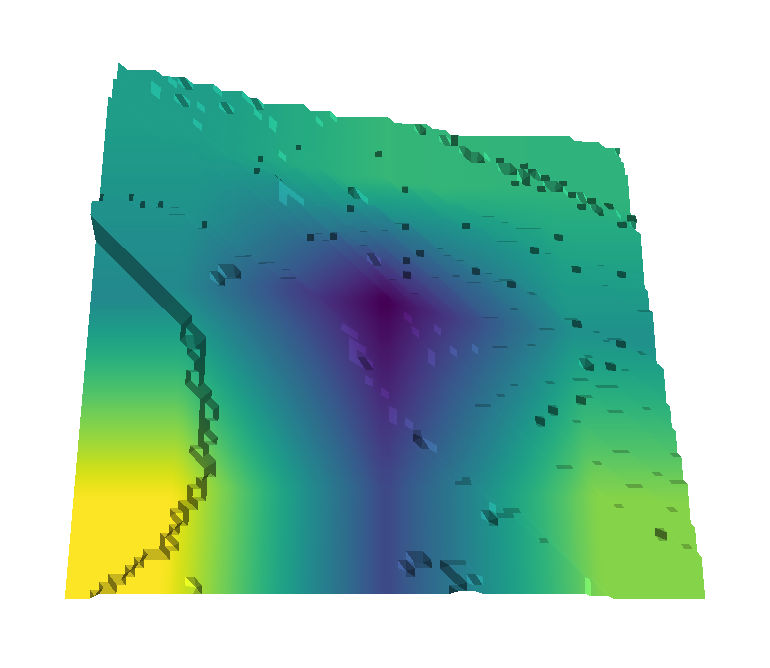
\includegraphics[width=\linewidth]{../img/5/quarry/false_negative/00-patch-3d-majavi-colormap-40.png}
    \caption{-0.00cm}
    \label{fig : quarry-false_negative-5}
    \end{subfigure}
    \begin{subfigure}[b]{0.192\linewidth}
    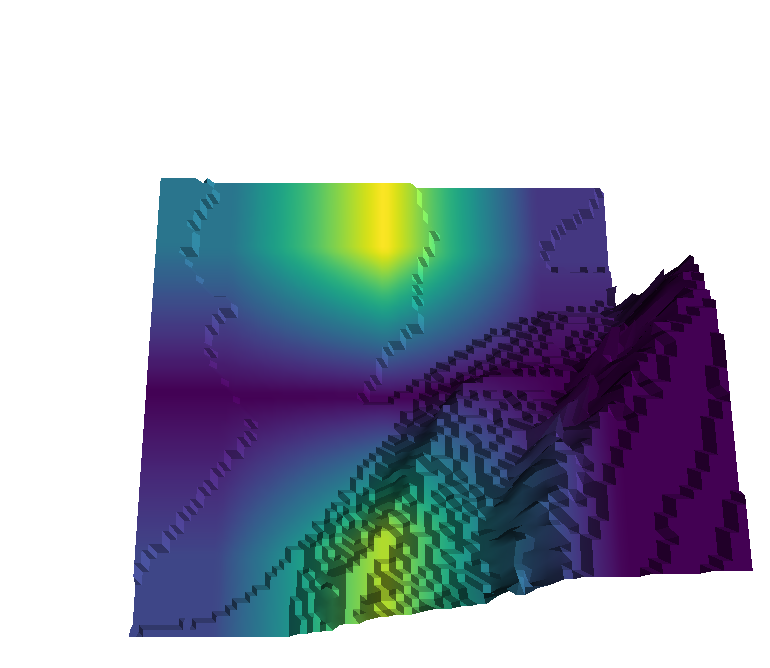
\includegraphics[width=\linewidth]{../img/5/quarry/false_negative/01-patch-3d-majavi-colormap-50.png}
    \caption{0.01cm}
    \label{fig : quarry-false_negative-6}
    \end{subfigure}
    \begin{subfigure}[b]{0.192\linewidth}
    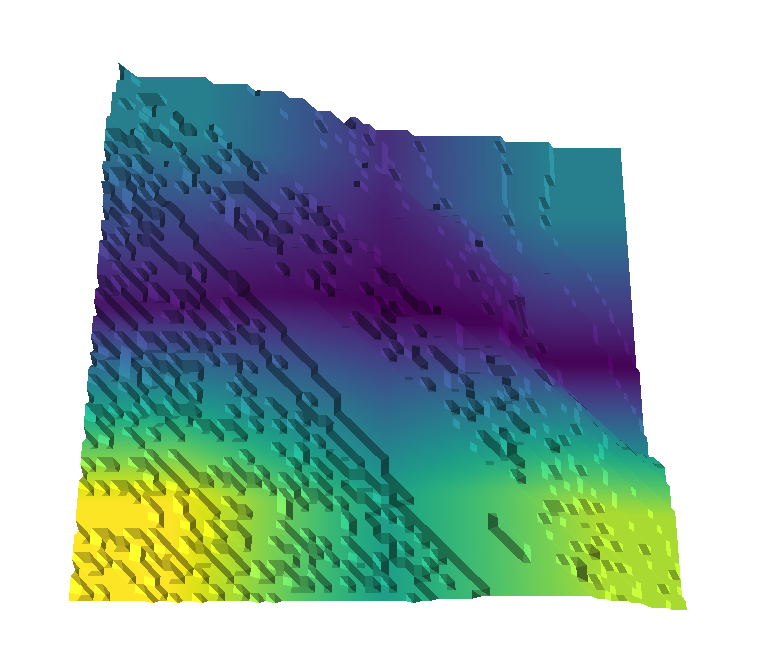
\includegraphics[width=\linewidth]{../img/5/quarry/false_negative/02-patch-3d-majavi-colormap-60.png}
    \caption{0.03cm}
    \label{fig : quarry-false_negative-7}
    \end{subfigure}
    \begin{subfigure}[b]{0.192\linewidth}
    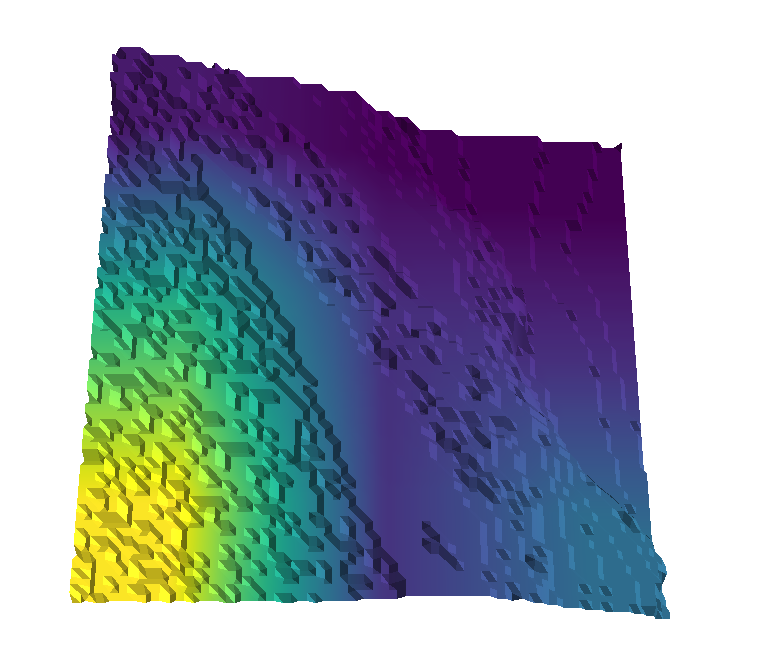
\includegraphics[width=\linewidth]{../img/5/quarry/false_negative/04-patch-3d-majavi-colormap-70.png}
    \caption{0.04cm}
    \label{fig : quarry-false_negative-8}
    \end{subfigure}
    \begin{subfigure}[b]{0.192\linewidth}
    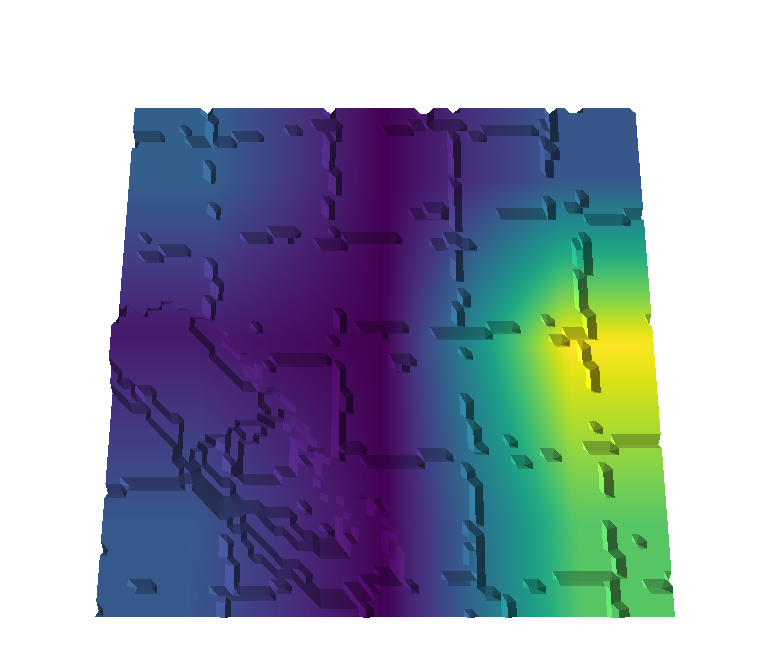
\includegraphics[width=\linewidth]{../img/5/quarry/false_negative/05-patch-3d-majavi-colormap-80.png}
    \caption{0.06cm}
    \label{fig : quarry-false_negative-9}
    \end{subfigure}
    \begin{subfigure}[b]{0.192\linewidth}
    \includegraphics[width=\linewidth]{../img/5/quarry/false_negative/06-patch-3d-majavi-colormap-90.png}
    \caption{0.07cm}
    \label{fig : quarry-false_negative-10}
    \end{subfigure}
    \begin{subfigure}[b]{0.192\linewidth}
    \includegraphics[width=\linewidth]{../img/5/quarry/false_negative/08-patch-3d-majavi-colormap-100.png}
    \caption{0.08cm}
    \label{fig : quarry-false_negative-11}
    \end{subfigure}
    \begin{subfigure}[b]{0.192\linewidth}
    \includegraphics[width=\linewidth]{../img/5/quarry/false_negative/09-patch-3d-majavi-colormap-110.png}
    \caption{0.09cm}
    \label{fig : quarry-false_negative-12}
    \end{subfigure}
    \begin{subfigure}[b]{0.192\linewidth}
    \includegraphics[width=\linewidth]{../img/5/quarry/false_negative/10-patch-3d-majavi-colormap-120.png}
    \caption{0.11cm}
    \label{fig : quarry-false_negative-13}
    \end{subfigure}
    \begin{subfigure}[b]{0.192\linewidth}
    \includegraphics[width=\linewidth]{../img/5/quarry/false_negative/11-patch-3d-majavi-colormap-130.png}
    \caption{0.12cm}
    \label{fig : quarry-false_negative-14}
    \end{subfigure}
    \begin{subfigure}[b]{0.192\linewidth}
    \includegraphics[width=\linewidth]{../img/5/quarry/false_negative/12-patch-3d-majavi-colormap-140.png}
    \caption{0.13cm}
    \label{fig : quarry-false_negative-15}
    \end{subfigure}
    \begin{subfigure}[b]{0.192\linewidth}
    \includegraphics[width=\linewidth]{../img/5/quarry/false_negative/14-patch-3d-majavi-colormap-150.png}
    \caption{0.14cm}
    \label{fig : quarry-false_negative-16}
    \end{subfigure}
    \begin{subfigure}[b]{0.192\linewidth}
    \includegraphics[width=\linewidth]{../img/5/quarry/false_negative/15-patch-3d-majavi-colormap-160.png}
    \caption{0.15cm}
    \label{fig : quarry-false_negative-17}
    \end{subfigure}
    \begin{subfigure}[b]{0.192\linewidth}
    \includegraphics[width=\linewidth]{../img/5/quarry/false_negative/16-patch-3d-majavi-colormap-170.png}
    \caption{0.17cm}
    \label{fig : quarry-false_negative-18}
    \end{subfigure}
    \begin{subfigure}[b]{0.192\linewidth}
    \includegraphics[width=\linewidth]{../img/5/quarry/false_negative/17-patch-3d-majavi-colormap-180.png}
    \caption{0.18cm}
    \label{fig : quarry-false_negative-19}
    \end{subfigure}
    \begin{subfigure}[b]{0.192\linewidth}
    \includegraphics[width=\linewidth]{../img/5/quarry/false_negative/18-patch-3d-majavi-colormap-190.png}
    \caption{0.18cm}
    \label{fig : quarry-false_negative-20}
    \end{subfigure}
    \label{fig : quarry-false_negative}
    \caption{Not traversable patches predicted as traversable sampled from the test dataset. We compute dthe Grad-CAM and applied as texture in the 3D render. The yellow highlights the ground region that contributed the most the model's prediction. }
    \end{figure}

\subsection{False positive patches}
False positive patches are the most interesting inputs. They are traversable patches classified as not. By looking at the features space, \ref{ fig :pca-test-patches}, we can noticed how the patches are mostly located close to the non traversable features. This explained why most of them are very close the surfaces presented before in figure \ref{fig : quarry-worst}. These samples included different types of terrains, some with obstacles ahead \ref{fig : false_positive-2}, \ref{fig : false_positive-3}, \ref{fig : false_positive-4}, \ref{fig : false_positive-7}, \ref{fig : false_positive-8}, \ref{fig : false_positive-11}, \ref{fig : false_positive-13}, \ref{fig : false_positive-14}, \ref{fig : false_positive-17}, \ref{fig : false_positive-19}, \ref{fig : false_positive-20}, slopes \ref{fig : false_positive-9}, \ref{fig : false_positive-10} and mixed grounds, \ref{fig : false_positive-1}, \ref{fig : false_positive-5}, \ref{fig : false_positive-12}, \ref{fig : false_positive-15}, \ref{fig : false_positive-16}, \ref{fig : false_positive-18}. In each case, the model identify meaningful features that can effect traversability. In the slopes, \ref{fig : false_positive-9} and \ref{false_positive-10}, the first part of the surface is highlighted. Similar to the traversable patches, the model tried to evaluated if the rear legs was able to move. This is also true for   \ref{fig : false_positive-6}. The only patch that consufed the model is the first one, \ref{fig : false_positive-18}, where it wrongly discriminated the flat region and not the obstacle. In all the others inputs, the network identifed importat region of the map that realistically could have caused the predicted not traversability.

\begin{figure}[H]
    \centering
    \begin{subfigure}[b]{0.192\linewidth}
    \includegraphics[width=\linewidth]{../img/5/quarry/false_positive/20-patch-3d-majavi-colormap-0.png}
    \caption{0.20cm}
    \label{fig : false_positive-1}
    \end{subfigure}
    \begin{subfigure}[b]{0.192\linewidth}
    \includegraphics[width=\linewidth]{../img/5/quarry/false_positive/20-patch-3d-majavi-colormap-12.png}
    \caption{0.21cm}
    \label{fig : false_positive-2}
    \end{subfigure}
    \begin{subfigure}[b]{0.192\linewidth}
    \includegraphics[width=\linewidth]{../img/5/quarry/false_positive/22-patch-3d-majavi-colormap-24.png}
    \caption{0.22cm}
    \label{fig : false_positive-3}
    \end{subfigure}
    \begin{subfigure}[b]{0.192\linewidth}
    \includegraphics[width=\linewidth]{../img/5/quarry/false_positive/23-patch-3d-majavi-colormap-36.png}
    \caption{0.23cm}
    \label{fig : false_positive-4}
    \end{subfigure}
    \begin{subfigure}[b]{0.192\linewidth}
    \includegraphics[width=\linewidth]{../img/5/quarry/false_positive/24-patch-3d-majavi-colormap-48.png}
    \caption{0.24cm}
    \label{fig : false_positive-5}
    \end{subfigure}
    \begin{subfigure}[b]{0.192\linewidth}
    \includegraphics[width=\linewidth]{../img/5/quarry/false_positive/25-patch-3d-majavi-colormap-60.png}
    \caption{0.25cm}
    \label{fig : false_positive-6}
    \end{subfigure}
    \begin{subfigure}[b]{0.192\linewidth}
    \includegraphics[width=\linewidth]{../img/5/quarry/false_positive/25-patch-3d-majavi-colormap-72.png}
    \caption{0.26cm}
    \label{fig : false_positive-7}
    \end{subfigure}
    \begin{subfigure}[b]{0.192\linewidth}
    \includegraphics[width=\linewidth]{../img/5/quarry/false_positive/26-patch-3d-majavi-colormap-84.png}
    \caption{0.27cm}
    \label{fig : false_positive-8}
    \end{subfigure}
    \begin{subfigure}[b]{0.192\linewidth}
    \includegraphics[width=\linewidth]{../img/5/quarry/false_positive/27-patch-3d-majavi-colormap-96.png}
    \caption{0.27cm}
    \label{fig : false_positive-9}
    \end{subfigure}
    \begin{subfigure}[b]{0.192\linewidth}
    \includegraphics[width=\linewidth]{../img/5/quarry/false_positive/27-patch-3d-majavi-colormap-108.png}
    \caption{0.28cm}
    \label{fig : false_positive-10}
    \end{subfigure}
    \begin{subfigure}[b]{0.192\linewidth}
    \includegraphics[width=\linewidth]{../img/5/quarry/false_positive/29-patch-3d-majavi-colormap-120.png}
    \caption{0.29cm}
    \label{fig : false_positive-11}
    \end{subfigure}
    \begin{subfigure}[b]{0.192\linewidth}
    \includegraphics[width=\linewidth]{../img/5/quarry/false_positive/30-patch-3d-majavi-colormap-132.png}
    \caption{0.30cm}
    \label{fig : false_positive-12}
    \end{subfigure}
    \begin{subfigure}[b]{0.192\linewidth}
    \includegraphics[width=\linewidth]{../img/5/quarry/false_positive/31-patch-3d-majavi-colormap-144.png}
    \caption{0.32cm}
    \label{fig : false_positive-13}
    \end{subfigure}
    \begin{subfigure}[b]{0.192\linewidth}
    \includegraphics[width=\linewidth]{../img/5/quarry/false_positive/33-patch-3d-majavi-colormap-156.png}
    \caption{0.34cm}
    \label{fig : false_positive-14}
    \end{subfigure}
    \begin{subfigure}[b]{0.192\linewidth}
    \includegraphics[width=\linewidth]{../img/5/quarry/false_positive/35-patch-3d-majavi-colormap-168.png}
    \caption{0.35cm}
    \label{fig : false_positive-15}
    \end{subfigure}
    \begin{subfigure}[b]{0.192\linewidth}
    \includegraphics[width=\linewidth]{../img/5/quarry/false_positive/36-patch-3d-majavi-colormap-180.png}
    \caption{0.36cm}
    \label{fig : false_positive-16}
    \end{subfigure}
    \begin{subfigure}[b]{0.192\linewidth}
    \includegraphics[width=\linewidth]{../img/5/quarry/false_positive/38-patch-3d-majavi-colormap-192.png}
    \caption{0.39cm}
    \label{fig : false_positive-17}
    \end{subfigure}
    \begin{subfigure}[b]{0.192\linewidth}
    \includegraphics[width=\linewidth]{../img/5/quarry/false_positive/41-patch-3d-majavi-colormap-204.png}
    \caption{0.41cm}
    \label{fig : false_positive-18}
    \end{subfigure}
    \begin{subfigure}[b]{0.192\linewidth}
    \includegraphics[width=\linewidth]{../img/5/quarry/false_positive/46-patch-3d-majavi-colormap-216.png}
    \caption{0.46cm}
    \label{fig : false_positive-19}
    \end{subfigure}
    \begin{subfigure}[b]{0.192\linewidth}
    \includegraphics[width=\linewidth]{../img/5/quarry/false_positive/51-patch-3d-majavi-colormap-228.png}
    \caption{0.52cm}
    \label{fig : false_positive-20}
    \end{subfigure}
    \label{fig : false_positive}
    \caption{Traversable patches predicted as not traversable sampled from the test dataset. We compute dthe Grad-CAM and applied as texture in the 3D render. The yellow highlights the ground region that contributed the most the model's prediction. }
    \end{figure}


% \end{document}